\documentclass[compress]{beamer}

%--------------------------------------------------------------------------
% Common packages
%--------------------------------------------------------------------------
\usepackage[english]{babel}
\usepackage{pgfpages} % required for notes on second screen
\usepackage{graphicx}
\usepackage{subfigure}
\usepackage{multicol}
\usepackage[normalem]{ulem}

\usepackage{tabularx,ragged2e}
\usepackage{booktabs}

%--------------------------------------------------------------------------
% Load theme
%--------------------------------------------------------------------------
\usetheme{hri}

\usepackage{tikz}
\usetikzlibrary{fpu,fit,calc,mindmap,backgrounds,positioning,svg.path}

\graphicspath{{figs/}}

% for model of anthopomorphism
\newcommand{\ICA}{{$\mathcal{A}_0$~}}
\newcommand{\SLA}{{$\mathcal{A}_\infty$~}}
\newcommand{\sla}{{\mathcal{A}_\infty}}
\newcommand{\AntMax}{{$\mathcal{A}_{max}$~}}
\newcommand{\antMax}{{\mathcal{A}_{max}}}

% for HATP plans
\newcommand{\hatpaction}[3]{#1\\\textsf{\scriptsize #2,}\\\textsf{\scriptsize #3}}

% for mutual modelling
\newcommand{\Mmodel}[3]{{\mathcal{M}(#1, #2, #3)}}
\newcommand{\model}[3]{{$\mathcal{M}(#1, #2, #3)$}}
\newcommand{\Model}[3]{{$\mathcal{M}^{\circ}(#1, #2, #3)$}}

% typeset logical concept
\newcommand{\concept}[1]{{\scriptsize \texttt{#1}}}

\newsavebox{\ontoinstance}
\savebox{\ontoinstance}{
\begin{tikzpicture}[
    >=latex,
    every edge/.style={<-, draw, very thick},
    every node/.style={draw, font=\sf, node distance=0.5, rounded corners,
    align=center, inner sep=5pt,fill=hriSec2Dark!50},
    classof/.style={<-, draw=black!60, dashed},
    property/.style={<-, draw=hriSec2Comp},
    propname/.style={above, draw=none, fill=none, font=\tt, inner sep=2pt},
    instance/.style={draw=hriSec1Dark, font=\sf, node distance=0.5, rounded corners,
align=center, inner sep=5pt, fill=none}]

    \node[fill=hriSec2Comp!50] (thing) {\textbf{thing}};
    \node [fill=hriSec3CompDark!50, node distance=1.8, below left=of
    thing](sthing) {place} edge[dashed] (thing);
    \node [fill=hriSec3CompDark!50, below left=of sthing] (agent) {agent} edge (sthing);
        \node [fill=hriSec3CompDark!50, below=of sthing] (artifact) {artifact} edge (sthing);
        \node [fill=hriSec3CompDark!50, below right=of sthing] (location) {physical
        support} edge (sthing);
        \node [fill=hriSec3CompDark!50, below right=of artifact] (table) {table}
            edge (location) edge (artifact);


    \node [node distance=1, below right=of thing] (tthing) {temporal thing} edge (thing);
        \node [below right=of tthing] (evt) {event} edge[dashed] (tthing);
                    \node [below right=of evt] (act) {action} edge (evt);

  \draw[dotted, thick] (-5,-5) -- (7.5, -5);

  \node [instance, below=3 of agent] (human) {human\_1} edge[classof, bend left] (agent);
  \node [instance, above right=of human, anchor=south] (robot) {pr2\_robot} edge[classof, bend left] (agent);
  \node [instance, right=of human, anchor=north west] (book) {book\_game\_thrones}
  edge[classof] (artifact);
  \node [instance, right=2 of robot] (ikea) {ikea\_table} edge[classof, bend
  right] (table);
  \node [instance, right=2 of book] (red) {red} edge[property] node[propname] {hasColor} (book);

  \draw[dotted, thick] (-5,-8) -- (7.5, -8);

  \path (book.200) edge [property, out=-100, in=-80, looseness=2]
  node[propname,auto] {isNextTo} (human.south);
  \path (book.270) edge [property, out=-100, in=-90, looseness=3.5] node[propname,auto] {looksAt} (robot.south);
  \path (ikea.south) edge [property, out=-90, in=-80, looseness=3] node[propname, auto] {isOn} (book.320);
\end{tikzpicture}
}


%--------------------------------------------------------------------------
% General presentation settings
%--------------------------------------------------------------------------
\title{Of Cognition and Social Robots}
\subtitle{Is ``Social Cognition'' in HRI just a buzz word?}
\date{Bristol Robotics Lab -- {\Medium \today}}
\author{Séverin Lemaignan}
\institute{Centre for Robotics and Neural Systems\\{\Medium
Plymouth University}}

%--------------------------------------------------------------------------
% Notes settings
%--------------------------------------------------------------------------
%\setbeameroption{show notes on second screen}
%\setbeameroption{hide notes}

\begin{document}

\maketitle

%%%%%%%%%%%%%%%%%%%%%%%%%%%%%%%%%%%%%%%%%%%%%%%%%%%%%%%%%%%%%%%%%%%%%%%%%%%%%%%
%%%%%%%%%%%%%%%%%%%%%%%%%%%%%%%%%%%%%%%%%%%%%%%%%%%%%%%%%%%%%%%%%%%%%%%%%%%%%%%
%%%%%%%%%%%%%%%%%%%%%%%%%%%%%%%%%%%%%%%%%%%%%%%%%%%%%%%%%%%%%%%%%%%%%%%%%%%%%%%


\begin{frame}[plain]{}

        \LARGE

        ``Cognition is a group of mental processes that includes {\Medium
        attention}, {\Medium memory}, producing and understanding {\Medium
        language}, {\Medium learning}, {\Medium reasoning}, {\Medium problem
        solving}, and {\Medium decision making}.''

\end{frame}

\begin{frame}[plain]{}

    \begin{multicols}{2}
        \resizebox{\columnwidth}{!}{%
        \vspace*{4cm}
        \begin{tikzpicture}
            
            \path[small mindmap, level 1 concept/.append style={sibling angle=360/7}, concept color=hriWarmGreyLight,text=hriWarmGreyDark]
            node[concept] {Cognition}
            [clockwise from=-30]
            child[concept color=hriSec2Dark,text=white] { node[concept]{Attention} }
            child[concept color=hriSec1CompDark,text=white] { node[concept] {Memory} }
            child[concept color=hriSec2CompDark,text=white] { node[concept] {Language} }
            child[concept color=hriSec3Comp,text=white] { node[concept] {Learning} }
            child[concept color=hriSec3CompDark,text=white] { node[concept] {Reasoning} }
            child[concept color=hriSec3Dark,text=white] { node[concept] {Problem solving} }
            child[concept color=hriSec1Dark,text=white] { node[concept] {Decision making} };
        \end{tikzpicture}
    }

    \begin{center}
        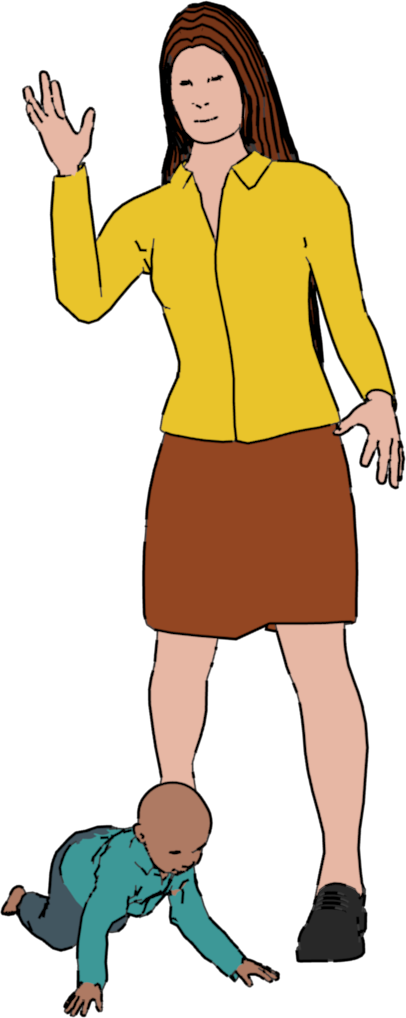
\includegraphics[width=0.4\columnwidth]{humans.png}
    \end{center}

    \end{multicols}

\end{frame}


\begin{frame}[plain]{}

    \begin{multicols}{2}
        \resizebox{1.3\columnwidth}{!}{%
            \begin{tikzpicture}[
                    >=latex,
                every edge/.style={<-, draw, very thick}]
        
            \path[small mindmap, 
                  level 1 concept/.append style={sibling angle=360/5}, 
                  level 2 concept/.append style={sibling angle=120}, 
                  concept color=hriWarmGreyLight,text=hriWarmGreyDark]
            node[concept] {Cognition}
            [clockwise from=-30]
            child[concept color=hriSec1,text=white] { node[concept] (percept) {Perception}
                [clockwise from=0]
                child[concept color=hriSec2Dark,text=white] { node[concept]{Attention} }
            }
            child[concept color=hriSec2Comp,text=white] { node[concept] (krr) {Knowledge Management} 
                [clockwise from=-30]
                child[concept color=hriSec1CompDark,text=white] { node[concept] {Memory} }
            }
            child[concept color=hriSec2,text=white] { node[concept] (action) {Action Execution} 
                [clockwise from=110]
                child[concept color=hriSec3,text=white] { node[concept] (plan) {Task Planning} }
            }
            child[concept color=hriSec3Comp,text=white] { node[concept] {Learning} }
            child[concept color=hriSec3CompDark,text=white] { node[concept] (reason) {Reasoning} 
                [clockwise from=100]
                child[concept color=hriSec3Dark,text=white] { node[concept] {Problem solving} }
            child[concept color=hriSec1Dark,text=white] { node[concept] (decision) {Decision making} } };

        \onslide<2>{
        \path (decision) edge[->, bend left] (action);
        \path (percept) edge[->, bend left] (action);
        \path (krr) edge[<->, bend right] (reason);
        \path (plan) edge[<->] (reason);
        \path (percept) edge[->, bend left] (krr);
        \path (krr) edge[->, bend left] (plan);
        }

        \end{tikzpicture}
    }

    \begin{center}
        \vspace*{1cm}
        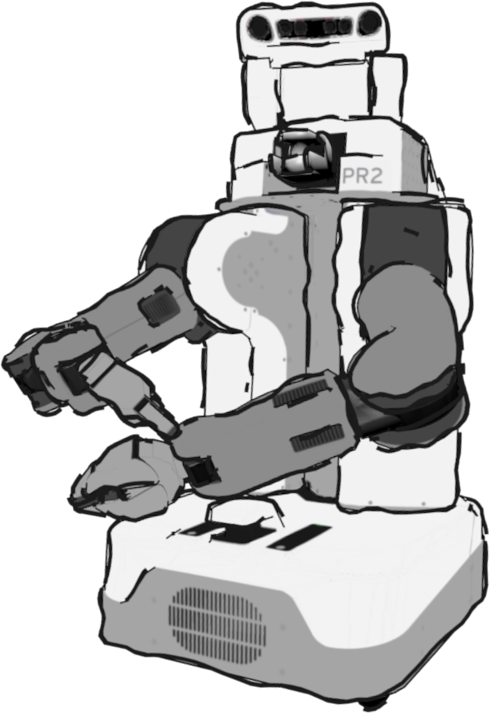
\includegraphics[width=0.6\columnwidth]{pr2.png}
    \end{center}

    \end{multicols}

\end{frame}


\begin{frame}[plain]{}

    \begin{multicols}{2}
        \resizebox{1.3\columnwidth}{!}{%
        \begin{tikzpicture}
            
            \path[small mindmap, 
                level 1 concept/.append style={sibling angle=360/5}, 
                level 2 concept/.append style={sibling angle=120}, 
            concept color=hriWarmGreyLight,text=hriWarmGreyDark]
            node[concept] {Cognition}
            [clockwise from=-30]
            child[concept color=hriSec1,text=white] { node[concept] (perception) {Perception}
                [clockwise from=40]
                child[concept color=hriSec2Dark,text=white] { node[concept]{Attention} }
                child[concept color=hriSec2CompDark,text=white] { node[concept] (dialog) {Communication} }
            }
            child[concept color=hriSec2Comp,text=white] { node[concept] (krr) {Knowledge Management} 
                [clockwise from=-30]
                child[concept color=hriSec1CompDark,text=white] { node[concept] {Memory} }
                child[concept color=hriSec3CompDark,text=white] { node[concept] (mmodel) {Mutual Modelling} }
            }
            child[concept color=hriSec2,text=white] { node[concept] {Action Execution} 
                [counterclockwise from=110]
                child[concept color=hriSec3,text=white] { node[concept] (plans) {Task Planning} }
                child[concept color=hriSec2CompDark,text=white] { node[concept] {Communication} }
            }
            child[concept color=hriSec3Comp,text=white] { node[concept] {Learning} 
                [counterclockwise from=130]
                child[concept color=hriSec1CompDark,text=white] { node[concept] (adapt) {Adaptation} }
            }
            child[concept color=hriSec3CompDark,text=white] { node[concept] {Reasoning} 
                [clockwise from=110]
                child[concept color=hriSec3Dark,text=white] { node[concept] {Problem solving} }
                child[concept color=hriSec1Dark,text=white] { node[concept] {Decision making} } 
            };

        \end{tikzpicture}
    }

    \begin{center}
        \vspace*{1cm}
        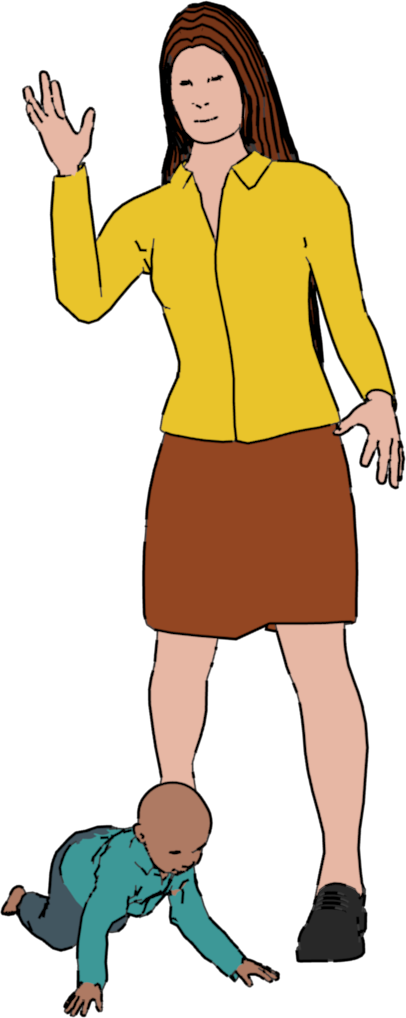
\includegraphics[width=0.4\columnwidth]{humans.png}
        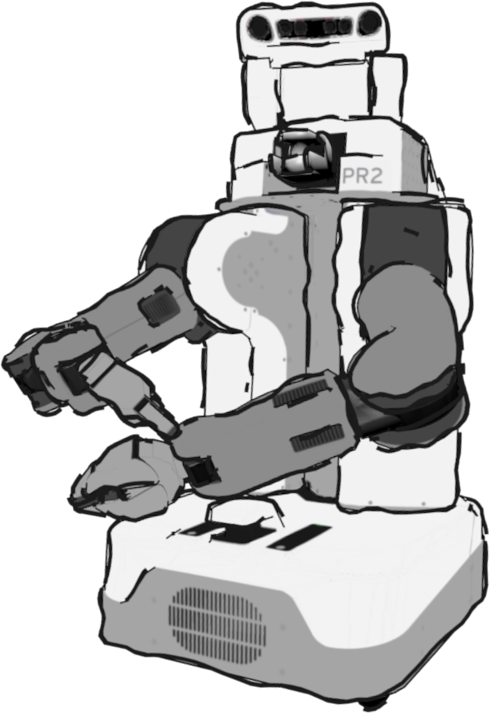
\includegraphics[width=0.5\columnwidth]{pr2.png}
    \end{center}

    \end{multicols}

\end{frame}


\begin{frame}[plain]{}
\centering
        \resizebox{!}{0.7\paperheight}{%
            \begin{tikzpicture}[
                    >=latex,
                every edge/.style={<-, draw, very thick}]
        

            \path[small mindmap, 
                level 1 concept/.append style={sibling angle=360/5}, 
                level 2 concept/.append style={sibling angle=120}, 
            concept color=hriWarmGreyLight,text=hriWarmGreyDark]
            node[concept] {Cognition}
            [clockwise from=-30]
            child[concept color=hriSec1,text=white] { node[concept] (percept) {Perception}
                [clockwise from=40]
                child[concept color=hriSec2Dark,text=white] { node[concept]{Attention} }
                child[concept color=hriSec2CompDark,text=white] { node[concept] (dialog) {Communication} }
            }
            child[concept color=hriSec2Comp,text=white] { node[concept] (krr) {Knowledge Representation} 
                [clockwise from=-30]
                child[concept color=hriSec1CompDark,text=white] { node[concept] (memory) {Memory} }
                child[concept color=hriSec3CompDark,text=white] { node[concept] (tom) {Theory of Mind} }
            }
            child[concept color=hriSec2,text=white] { node[concept] (action) {Action Execution} 
                [counterclockwise from=110]
                child[concept color=hriSec3,text=white] { node[concept] (plan) {Task Planning} }
                child[concept color=hriSec2CompDark,text=white] { node[concept] (comm) {Communication} }
            }
            child[concept color=hriSec3Comp,text=white] { node[concept] (learning) {Learning} 
                [counterclockwise from=130]
                child[concept color=hriSec1CompDark,text=white] { node[concept] (adapt) {Adaptation} }
            }
            child[concept color=hriSec3CompDark,text=white] { node[concept] (reason) {Reasoning} 
                [clockwise from=110]
                child[concept color=hriSec3Dark,text=white] { node[concept] {Problem solving} }
                child[concept color=hriSec1Dark,text=white] { node[concept] (decision) {Decision making} } 
            };

        \path (decision) edge[->, bend left] (action);
        \path (percept) edge[->, bend left] (action);
        \path (krr) edge[<->, bend right] (reason);
        \path (plan) edge[<->] (reason);
        \path (percept) edge[->, bend left] (krr);
        \path (krr) edge[->, bend left] (plan);
        \path (learning) edge[->, bend left] (reason);
        \path (learning) edge[->, bend left] (krr);
        \path (percept) edge[<->, bend left] (learning);
        \path (dialog) edge[->, bend left] (tom);
        \path (tom) edge[->, bend left] (comm);
        \path (percept) edge[<->, bend left] (memory);


        \end{tikzpicture}
    }
\end{frame}

{
\paper{Baxter, Lemaignan, Trafton {\Medium Workshop on Cognitive Architectures for Social HRI} -- HRI 2016}
\begin{frame}{Functions for Social Cognition}
\centering
        \resizebox{!}{0.7\paperheight}{%
            \begin{tikzpicture}[
                    >=latex,
                every edge/.style={<-, draw, very thick}]
        

            \path[small mindmap, 
                level 1 concept/.append style={sibling angle=360/6}, 
                level 2 concept/.append style={sibling angle=60}, 
            concept color=white,text=hriWarmGreyDark]
            node[concept] {\Medium Social\\Cognition in HRI}
            [clockwise from=30]
            child[concept color=hriSec1,text=white] { node[concept] (percept) {Perception of Human's State}
                [clockwise from=120]
                child[concept color=hriSec3Dark,text=white] { node[concept]{Emotions} }
                child[concept color=hriSec2Dark,text=white] { node[concept]{Attention} }
                child[concept color=hriSec2CompDark,text=white] { node[concept]
                {Inference of mental models} };
            }
            child[concept color=hriSec2Comp,text=white,grow=-30] { node[concept] (knowledge) {Social Knowledge} 
                [counterclockwise from=-120]
                child[concept color=hriSec1CompDark,text=white] { node[concept] {Social rules} }
                child[concept color=hriSec3Comp,text=black] { node[concept] {Social context} }
                child[concept color=hriSec3CompDark,text=white] { node[concept]
                {Common-sense} };
            }
            child[concept color=hriSec3Comp,text=black, grow=-120] { node[concept] (comm) {Communication} 
                [counterclockwise from=180]
                child[concept color=hriSec1CompDark,text=white] { node[concept] {Verbal} }
                child[concept color=hriSec1Dark,text=white] { node[concept]
                {Non-verbal} };
            }
            child[concept color=hriSec3,text=white,grow=180] { node[concept] (dynamics) {Interaction Dynamics} 
                [clockwise from=180]
                child[concept color=hriSec2Dark,text=white] { node[concept]
                {Long-term interaction} };
            }
            child[concept color=hriSec2,text=black, grow=120] { node[concept]
                (action) {Performing with humans} 
                [counterclockwise from=80]
                child[concept color=hriSec2CompDark,text=white] { node[concept] {Action, behaviour recognition} }
                child[concept color=hriSec1Dark,text=white] { node[concept] {Intention reading} }
                child[concept color=hriSec3,text=white] { node[concept] {Joint
                actions} };
            };

%                \node[circle, draw=red, very thick, minimum size=1.6cm] at (mmodel.center) {};
%                \node[circle, draw=red, very thick, minimum size=1.6cm] at (adapt.center) {};
%                \node[circle, draw=red, very thick, minimum size=1.6cm] at (plans.center) {};
%                \node[circle, draw=red, very thick, minimum size=2cm] at (krr.center) {};
%                \node[circle, draw=red, very thick, minimum size=2cm] at (perception.center) {};
%
%                \node[circle, dashed, draw=red, thick, minimum size=1.6cm] at (dialog.center) {};
%

        \end{tikzpicture}
    }
%    \\
%    Learn -- Memorize -- Reason -- Represent -- Assess Situation
\end{frame}
}

%%%%%%%%%%%%%%%%%%%%%%%%%%%%%%%%%%%%%%%%%%%%%%%%%%%%%%%%%%%%%%%%%%%%%%%%%%%%%%%
%%%%%%%%%%%%%%%%%%%%%%%%%%%%%%%%%%%%%%%%%%%%%%%%%%%%%%%%%%%%%%%%%%%%%%%%%%%%%%%
%%%%%%%%%%%%%%%%%%%%%%%%%%%%%%%%%%%%%%%%%%%%%%%%%%%%%%%%%%%%%%%%%%%%%%%%%%%%%%%


\section*{Overview}
\begin{frame}{Overview}
    \tableofcontents[hideallsubsections]
    %\tableofcontents
\end{frame}



%%%%%%%%%%%%%%%%%%%%%%%%%%%%%%%%%%%%%%%%%%%%%%%%%%%%%%%%%%%%%%%%%%%%%%%%%%%%%%%
%%%%%%%%%%%%%%%%%%%%%%%%%%%%%%%%%%%%%%%%%%%%%%%%%%%%%%%%%%%%%%%%%%%%%%%%%%%%%%%
%%%%%%%%%%%%%%%%%%%%%%%%%%%%%%%%%%%%%%%%%%%%%%%%%%%%%%%%%%%%%%%%%%%%%%%%%%%%%%%

\section{Represent}

\imageframe{pr2-baby-1.jpg}
\imageframe{pr2-baby-2.jpg}
\imageframe{pr2-baby-3.jpg}
\imageframe{pr2-baby-4.jpg}
%\imageframe[\scriptsize \Medium Mix of geometry, time, semantics\\ \vspace*{1em}
%        High geometric/temporal granularity (e.g. nodding)\\ \vspace*{1em}
%        Lots of common-sense knowledge, cultural background\\ \vspace*{1em}
%        %Non-monotonic topology\\
%        %Represent continuous/discrete fields\\
%        Account for uncertainties\\ \vspace*{1em}
%        %Imagine entities\\
%        Remember the past, imagine the future\\
%        %Temporal template matching, chronicles\\
% ]{pr2-baby-4.jpg}


\begin{frame}{Representation}
    Building robotic qualia: ``what it is like for the robot to experience...''
    \begin{enumerate}
        \item From situation assessment...
        \item ...to symbolic models...
        \item ...to perspective taking...
        \item ...to(wards) mutual modelling
   \end{enumerate}

\end{frame}


\subsection{From Spatial to Symbolic Models}
\begin{frame}{Situation Assessment}
        \centering
        \video{0.7\textwidth}{videos/model3d.webm?autostart&start=22}\\
        \vspace*{1em}
        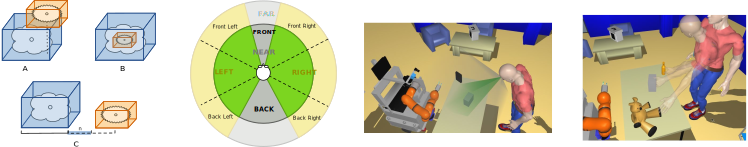
\includegraphics[width=0.9\textwidth]{spark.pdf}

\end{frame}

\begin{frame}{}
        \centering
        \scriptsize

        \begin{tabular}{p{1.5cm}lp{2cm}}
            Subject & Predicate  & Object  \\ 
            \hline
            \concept{Location} & \concept{isAt} $\equiv$ \concept{cyc:objectFoundInLocation}  &  \concept{Location}  \\ 
                               &  $\rightarrow$ \concept{isOn} $\equiv$ \concept{cyc:above\_Touching}  &   \\ 
                               &  $\rightarrow$ \concept{isIn}  &   \\ 
                               &  $\rightarrow$ \concept{isNextTo}  &   \\ 

            \concept{Location}  & \concept{isAbove} $\equiv$ \concept{cyc:above-Generally}  &  \concept{Location} \\ 
            \concept{Location}  & \concept{isBelow}  & \concept{Location} \\
            \hline
            \concept{Location}  & \concept{hasRelativePosition}  & \concept{Location}  \\ 
                                   & 	$\rightarrow$ \concept{behind} $\equiv$ \concept{cyc:behind-Generally}  & \\ 
                                      &  $\rightarrow$ \concept{inFrontOf} $\equiv$ \concept{cyc:inFrontOf-Generally}  & \\ 
                                         &  $\rightarrow$ \concept{leftOf}  &  \\ 
                                            &  $\rightarrow$ \concept{rightOf}  & 	 \\ 
            \concept{Object}  & \concept{cyc:farFrom}  &  \concept{Agent} \\ 
            \concept{Object}  & \concept{cyc:near}  &  \concept{Agent} \\

            \hline
            \concept{Agent}  & \concept{looksAt}  & \concept{SpatialThing} \\
            \concept{Agent}  & \concept{sees}  &  \concept{SpatialThing}  \\ 
            \concept{SpatialThing}  & \concept{isInFieldOfView}  & \concept{xsd:boolean}  \\ 
            \concept{Agent}  & \concept{pointsAt} $\equiv$ \concept{cyc:pointingToward}  & \concept{SpatialThing} \\ 
            \concept{Agent}  & \concept{focusesOn}  &  \concept{SpatialThing}  \\ 
            \concept{Agent} & \concept{seesWithHeadMovement} &  \concept{SpatialThing} \\
            \concept{Agent} & \concept{canReach} &  \concept{Object} \\ 

        \end{tabular}

\end{frame}

\begin{frame}{From Spatial Model to Symbolic Model}

    \begin{figure}
        \centering

        \resizebox{0.9\paperwidth}{!}{%
            \begin{tikzpicture}[
                    >=latex,
                    every edge/.style={<-, draw, very thick},
                    every node/.style={draw, font=\sf, node distance=0.5, rounded corners,
                align=center, inner sep=5pt,fill=hriSec2Dark!50}]

                \node[fill=hriSec2Comp!50] (thing) {\Medium thing};
                \node [fill=hriSec3CompDark!50, node distance=1.8, below left=of thing](sthing) {spatial thing} edge (thing);
                \node [fill=hriSec3CompDark!50, above left=of sthing] {posture} edge (sthing);
                \node [fill=hriSec3CompDark!50, left=of sthing] {shape} edge (sthing);
                \node [fill=hriSec3CompDark!50, below=of sthing] (location) {location} edge (sthing);
                \node [fill=hriSec3CompDark!50, below right=of location] {zone} edge (location);
                \node [fill=hriSec3CompDark!50, below left=of location] (set) {spatial enduring thing} edge (location);
                \node [fill=hriSec3CompDark!50, below right=of set] {obstacle} edge (set);
                \node [fill=hriSec3CompDark!50, below left=of set] {opening} edge (set);
                \node [fill=hriSec3CompDark!50, below=1 of set] {partially tangible thing} edge (set);
                \node [fill=hriSec3CompDark!50, above left=of set] {place} edge (set);

                \node [node distance=1, below right=of thing] (tthing) {temporal thing} edge (thing);
                \node [below=of tthing] (tte) {thing with temporal extent} edge (tthing);
                \node [below right=of tte] {time interval} edge (tte);
                \node [below=1 of tte] (sit) {situation} edge (tte);
                \node [below right=of sit] (evt) {event} edge (sit);
                \node [below right=of evt] (act) {action} edge (evt);
                \node [below=of act] {purposeful action} edge (act);
                \node [below left=of sit] {static situation} edge (sit);

            \end{tikzpicture}
        }

    \end{figure}

\end{frame}

{
\paper{Lemaignan, Alami, {\Medium Explicit Knowledge and the Deliberative Layer: Lessons Learned}, IROS 2013}
\begin{frame}{Online Instantiation}

    \begin{multicols}{2}
        \centering
        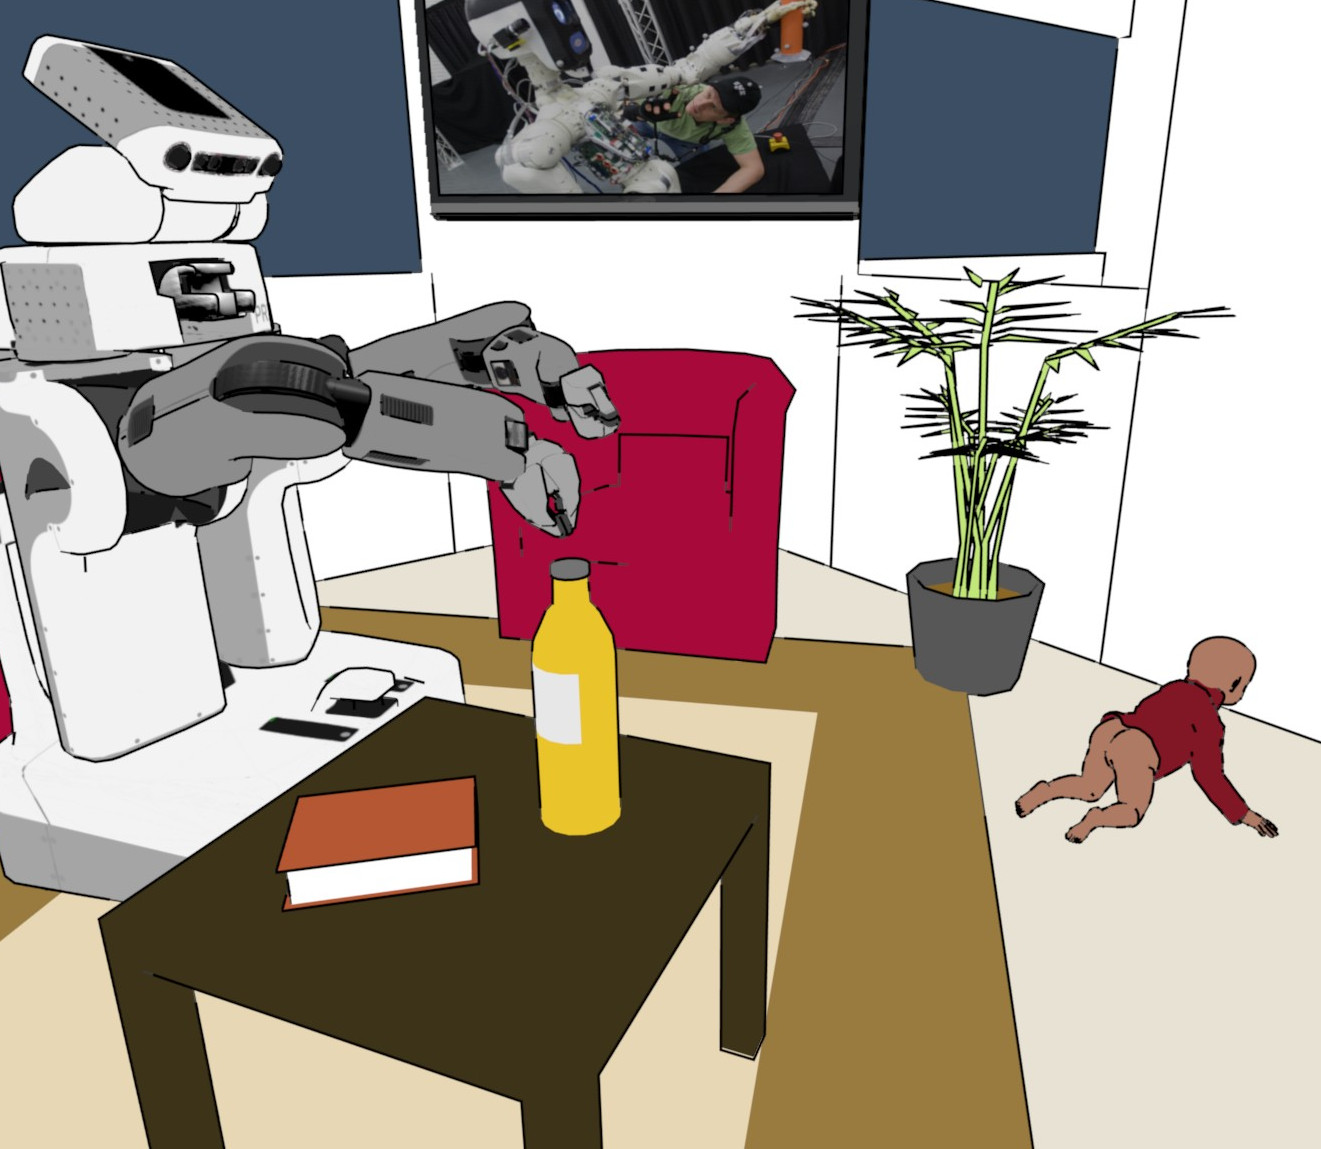
\includegraphics[width=\columnwidth]{pr2-scene.jpg}
        
        \begin{figure}

        \resizebox{\columnwidth}{!}{%
        \begin{tikzpicture}[
            yscale=1.3,
            >=latex,
            every edge/.style={<-, draw, very thick},
            every node/.style={draw, font=\sf, node distance=0.5, rounded corners,
            align=center, inner sep=5pt,fill=hriSec2Dark!50},
            classof/.style={<-, draw=black!60, dashed},
            property/.style={<-, draw=hriSec2Comp},
            propname/.style={above, draw=none, fill=none, font=\tt, inner sep=2pt},
            instance/.style={draw=hriSec1Dark, font=\sf, node distance=0.5, rounded corners,
        align=center, inner sep=5pt, fill=none}]

            \node[fill=hriSec2Comp!50] (thing) {\textbf{thing}};
            \node [fill=hriSec3CompDark!50, node distance=1.8, below left=of
            thing](sthing) {place} edge[dashed] (thing);
            \node [fill=hriSec3CompDark!50, below left=of sthing] (agent) {agent} edge (sthing);
                \node [fill=hriSec3CompDark!50, below=of sthing] (artifact) {artifact} edge (sthing);
                \node [fill=hriSec3CompDark!50, below right=of sthing] (location) {physical
                support} edge (sthing);
                \node [fill=hriSec3CompDark!50, below right=of artifact] (table) {table}
                    edge (location) edge (artifact);


            \node [node distance=1, below right=of thing] (tthing) {temporal thing} edge (thing);
                \node [below right=of tthing] (evt) {event} edge[dashed] (tthing);
                            \node [below right=of evt] (act) {action} edge (evt);

        \uncover<2->{
        \draw[dotted, thick] (-5,-3.8) -- +(13, 0);

        \node [instance, below=3 of agent] (human) {baby\_1} edge[classof, bend left] (agent);
        \node [instance, above right=of human, anchor=south] (robot) {pr2\_robot} edge[classof, bend left] (agent);
        \node [instance, right=of human, anchor=north west] (book) {book\_game\_thrones}
        edge[classof] (artifact);
        \node [instance, right=2 of robot] (ikea) {ikea\_table} edge[classof, bend
        right] (table);
        \node [instance, right=2 of book] (brown) {brown} edge[property] node[propname] {hasColor} (book);


        }
        \uncover<3>{
        \draw[dotted, thick] (-5,-6.2) -- +(13, 0);

        \node [instance, below=5 of act] (moving) {move\_act\_42} edge[classof] (act);
        \path (moving.west) edge [property, out=180, in=-80, looseness=1] node[propname,below] {currentlyPerforms} (human.230);
        \path (human.280) edge [property, out=-80, in=-90, looseness=3.5] node[propname,right] {looksAt} (robot.south);
        \path (ikea.south) edge [property, out=-90, in=-80, looseness=3] node[propname, auto] {isOn} (book.320);
        }
        \end{tikzpicture}
        }

        \end{figure}

    \end{multicols}


\end{frame}
}

\videoframe[0.56]{videos/this_box.webm?autostart&start=1}

{
    \paper{Lemaignan et al. {\Medium Grounding the Interaction: Anchoring Situated Discourse in Everyday HRI} -- Intl. J. of Social Robotics 2011}
    \begin{frame}{}
        \centering
        I keep the natural language processing part for the questions, but:\\

        \vspace*{2em}
        ``Where is the other tape?''\\
        $\downarrow$\\
        find({\tt\scriptsize ?obj isAt ?loc, ?obj type VideoTape, ?obj differentFrom JIDO-E})
    \end{frame}
}





%%%%%%%%%%%%%%%%%%%%%%%%%%%%%%%%%%%%%%%%%%%%%%%%%%%%%%%%%%%%%%%%%%%%%%%%%%%%%%%
%%%%%%%%%%%%%%%%%%%%%%%%%%%%%%%%%%%%%%%%%%%%%%%%%%%%%%%%%%%%%%%%%%%%%%%%%%%%%%%
%%%%%%%%%%%%%%%%%%%%%%%%%%%%%%%%%%%%%%%%%%%%%%%%%%%%%%%%%%%%%%%%%%%%%%%%%%%%%%%

\section{Modelling the Other}

%%%%%%%%%%%%%%%%%%%%%%%%%%%%%%%%%%%%%%%%%%%%%%%%%%%%%%%%%%%%%%%%%%%%%%%%%%%%%%%

\subsection{Perspective Taking and Symbolic Modelling}

\imageframe{humans-pt}

\begin{frame}{Visual Perspective taking}
        \centering
        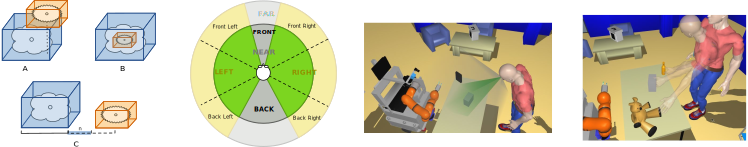
\includegraphics[width=0.9\textwidth]{spark.pdf}
        \vspace*{1em}
        \video{0.7\textwidth}{videos/talking_to_my_robot.mp4?start=84&stop=136&noaudio}

\end{frame}


{
\paper{Ros, Lemaignan et al., {\Medium Which One? Grounding the Referent Based on Efficient HRI}, ROMAN 2010}
\begin{frame}{Multiple Symbolic Models}
        \begin{multicols}{2}
            \begin{figure}
                \resizebox{0.35\textwidth}{!}{\usebox{\ontoinstance}}
            \end{figure}
            \begin{figure}
                \resizebox{0.35\textwidth}{!}{\usebox{\ontoinstance}}
            \end{figure}
            \begin{figure}
                \resizebox{0.35\textwidth}{!}{\usebox{\ontoinstance}}
            \end{figure}
            {\vspace*{1.5cm}\hspace*{2.5cm}\huge...}
        \end{multicols}
\end{frame}
}


\videoframe[0.56]{videos/dialogs.webm?autostart&stop=28}

{
    \paper{Lemaignan, Alami {\Medium Talking to my Robot: from Knowledge Grounding to Dialogue Processing} -- HRI 2013}
    \begin{frame}{}
        \centering

        \vspace*{2em}
        ``Give me the can!''\\
        $\downarrow$\\
        find({\tt\scriptsize ?obj type Can, model='severin'})
    \end{frame}
}


\subsection{Theory of Mind?}

\begin{frame}{The False-Belief Experiment}
    \centering
    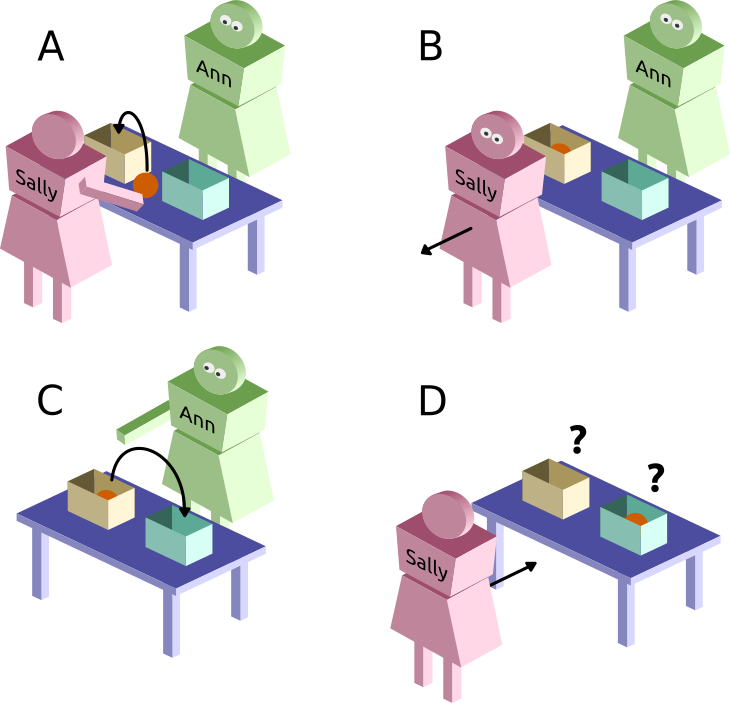
\includegraphics[width=0.7\textwidth]{sally_ann.pdf}

\end{frame}

{
    \paper{Warnier et al., {\Medium When the Robot Puts Itself in Your Shoes}, ROMAN 2012}
    \begin{frame}{The False-Belief Experiment}
        \centering
        \video{0.9\textwidth}{videos/falsebeliefs.webm?autostart}

    \end{frame}
}

{
    \paper{Frith and Happé {\Medium Autism: Beyond "theory of mind"} -- Cognition, 1994]\newline
           [Lemaignan, Dillenbourg {\Medium Mutual Modelling in Robotics: Inspirations for the Next Steps} -- HRI 2015}
\begin{frame}{Shopping list for HRI?}
    \centering
    \begin{tabular}{p{0.5\linewidth}p{0.5\linewidth}}
        \toprule
        {\Medium Already in the HRI fridge} & {\Medium To buy...} \\
        \midrule
        Instrumental gestures & Expressive gestures \\
        Using person as tool & Using person as receiver of information \\
        Talking about desires and emotions & Talking about beliefs and ideas \\
        Showing "active" sociability & Showing "interactive" sociability \\
        Elicited structured play & Spontaneous pretend play \\
        \bottomrule
    \end{tabular}
\end{frame}
}


{
    \paper{Frith and Happé {\Medium Autism: Beyond "theory of mind"} -- Cognition, 1994]\newline
           [Lemaignan, Dillenbourg {\Medium Mutual Modelling in Robotics: Inspirations for the Next Steps} -- HRI 2015}
\begin{frame}{Autistic assets and deficits observed in real life}
    \centering
    \begin{tabular}{p{0.5\linewidth}p{0.5\linewidth}}
        \toprule
        {\Medium Assets} & {\Medium Deficits} \\
        \midrule
        Instrumental gestures & Expressive gestures \\
        Using person as tool & Using person as receiver of information \\
        Talking about desires and emotions & Talking about beliefs and ideas \\
        Showing "active" sociability & Showing "interactive" sociability \\
        Elicited structured play & Spontaneous pretend play \\
        \bottomrule
    \end{tabular}
\end{frame}
}

%%%%%%%%%%%%%%%%%%%%%%%%%%%%%%%%%%%%%%%%%%%%%%%%%%%%%%%%%%%%%%%%%%%%%%%%%%%%%%%
\subsection{CoWriter}

\begin{frame}[plain]{}
    \centering
    Mind modelling is {\Medium mutual}
    
    We can take advantage of it in HRI at fundamental levels

\end{frame}
{
    \paper{Lemaignan et al. {\Medium Learning by Teaching a Robot: The Case of Handwriting} -- Robotics and Automation Magazine 2016}
\begin{frame}{CoWriter: cognitive engagement and meta-cognition}
    \video{0.55\textwidth}{videos/cowriter-session1_3minExcerpt_1x.mp4}

    \begin{flushright}
        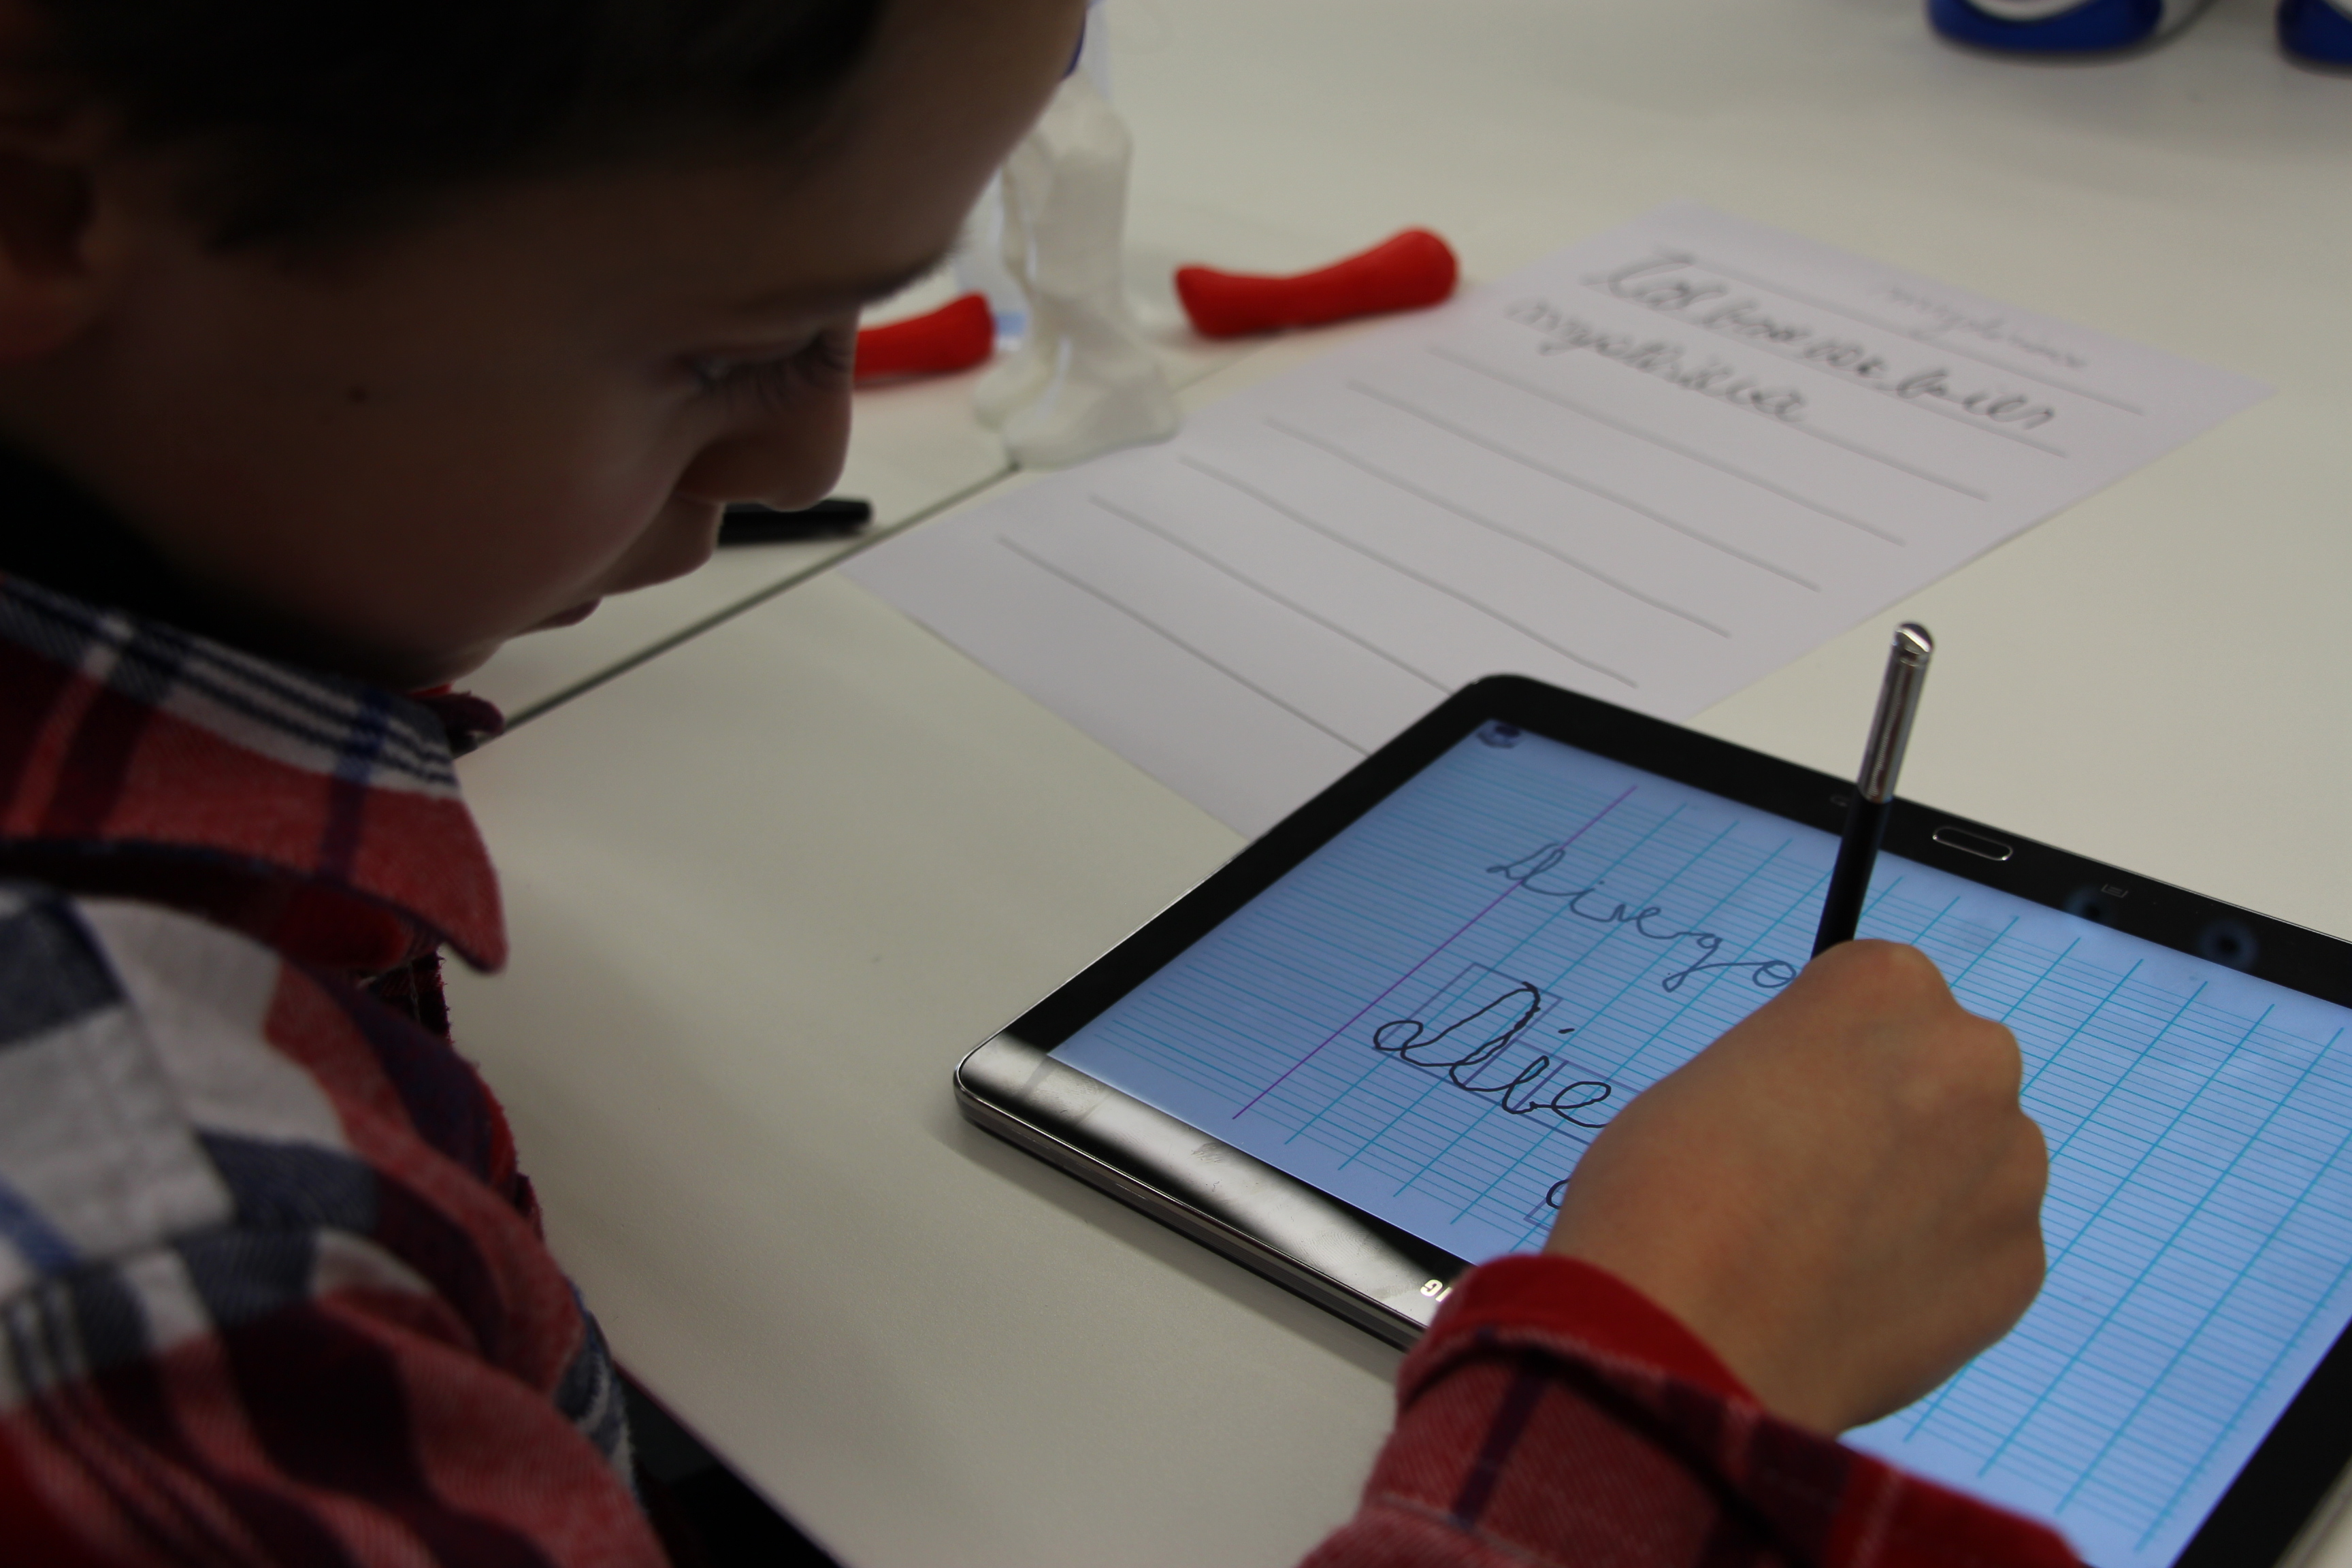
\includegraphics[width=0.5\textwidth]{diego-writing}
    \end{flushright}

\end{frame}
}

{
    \paper{Lemaignan et al. {\Medium Learning by Teaching a Robot: The Case of Handwriting} -- Robotics and Automation Magazine 2016}
\begin{frame}{}
    \begin{center}
        \includegraphics[width=0.45\linewidth]{lettre-base}
        \uncover<2>{
        \includegraphics[width=0.45\linewidth]{lettre-final}
    }
    \end{center}
\end{frame}
}


%%%%%%%%%%%%%%%%%%%%%%%%%%%%%%%%%%%%%%%%%%%%%%%%%%%%%%%%%%%%%%%%%%%%%%%%%%%%%%%%%
%%%%%%%%%%%%%%%%%%%%%%%%%%%%%%%%%%%%%%%%%%%%%%%%%%%%%%%%%%%%%%%%%%%%%%%%%%%%%%%%%
%%%%%%%%%%%%%%%%%%%%%%%%%%%%%%%%%%%%%%%%%%%%%%%%%%%%%%%%%%%%%%%%%%%%%%%%%%%%%%%%%


\section{Are you still with me?}
%%%%%%%%%%%%%%%%%%%%%%%%%%%%%%%%%%%%%%%%%%%%%%%%%%%%%%%%%%%%%%%%%%%%%%%%%%%%%%%%%

%%%%%%%%%%%%%%%%%%%%%%%%%%%%%%%%%%%%%%%%%%%%%%%%%%%%%%%%%%%%%%%%%%%%%%%%%%%%%%%%%
\subsection{Dynamics of Interaction}

{
\paper{Lemaignan, Fink, Dillenbourg, Braboszcz {\Medium The Cognitive Correlates of Anthropomorphism}, HRI 2014}
\begin{frame}{How do we perceive robot over time?}
    \begin{figure}
        \centering

        \resizebox{0.9\paperwidth}{!}{

            \begin{tikzpicture}

                % background shading
                \path[fill=hriSec2!50] (0,0) rectangle (0.6,5.5);
                \path[fill=hriSec1Comp!50] (0.6,0) rectangle (5.2,5.5);
                \path[fill=hriSec3Comp!50] (5.2,0) rectangle (9.8,5.5);
                \draw(0,5.5) node[anchor=south west, rotate=10] {\scriptsize \sc Initialization};
                \draw(2.5,5.5) node[anchor=south west, rotate=10] {\scriptsize \sc Familiarization};
                \draw(6.5,5.5) node[anchor=south west, rotate=10] {\scriptsize \sc Stabilization};
                % horizontal axis
                \draw[->] (0,0) -- (10,0) node[anchor=north] {$t$};
                \draw(5,-0.1) node[anchor=north] {\scriptsize Duration of interaction};


                % vertical axis
                \draw[->] (0,0) -- (0,6) node[anchor=east] {};
                \draw(-0.8,3) node[rotate=90,anchor=south] {\scriptsize Anthropomorphic effects};

                \draw (-0.05, 3) -- (0.05, 3) node[anchor=east] {\ICA};
                \draw (-0.05, 5) -- (0.05, 5) node[anchor=east] {\AntMax};

                % vertical axis - end
                \draw[->] (9.8,0) -- (9.8,2) node[anchor=east] {};
                \draw (9.8, 0.8) node[anchor=west] {\SLA};


                \draw[<-] (0.65,5) -- (0.8,5.2) node[anchor=east] {};
                \draw (0.9,5.3) node[anchor=west] {\tiny \it novelty peak};

                \draw[dashed] (0.6, 0) -- (0.6,5.1);
                \draw (0.6,0) node[anchor=north] {$t_{max}$};

                \draw[dotted] (0, 5) -- (6.2,5);
                \draw[dotted] (0, 3) -- (6.2,3);
                \draw[<->] (6.1,3) -- (6.1,5) node[sloped, above, midway] {$\Delta_{a}$};

                \draw[<-] (1.7,4.4) -- (3.2,4.1) node[anchor=east] {};
                \draw[<-] (2.85,2.6) -- (3.2,4.1) node[anchor=east] {};
                \draw (3.2,4.1) node[anchor=west, align=center] {\tiny \it disruptive\\ \tiny
                \it behaviors};
                %%%%%
                %% CURVES
                %%%%
                \begin{scope}[yscale=-1,shift={(-0.125,-0.4)}]

                    \draw[ultra thick] svg[scale=1cm] "M 0.125,-2.5619582 c 0.0200733,-1.1573591
                    0.33954391,-1.9982333 0.57940683,-2.0013597 0.13691605,0 0.25550329,0.052908
                    0.37497897,0.1661788 0.119476,0.1130305 0.2396954,0.2786079
                    0.37944,0.4790565 0.069872,0.099803 0.1021612,-0.2231749
                    0.1792538,-0.2238964 0.099707,0 0.013454,0.4985362 0.3173383,0.9139831
                    0.1911917,0.2612926 0.3444354,0.2578391 0.6711932,0.4894291
                    0.2058265,0.1458798 0.1571532,0.9762306 0.2615031,0.9702183 0.097182,0
                    0.083295,-0.3336208 0.4330446,-0.1199242 0.4306401,0.2631203
                    0.216699,0.1355642 0.4296663,0.2647074 2.0858202,1.13836043
                    4.34683,1.41300027 6.3741749,1.43753027";

                    \draw[dashed] svg[scale=1cm] "M 0.125,-0.1952939 c 0.0553601,-3.1917862
                    0.33954391,-4.3648976 0.57940683,-4.368024 0.13691605,0 0.25550329,0.052908
                    0.37497897,0.1661788 m 2.6714393,2.7735737 C 4.7653984,-0.85050947
                    6.5955093,0.35382293 10.125,0.4062498";

                    \draw[dashed] svg[scale=1cm] "M 0.125,-3.6923825 C 0.1102888,-4.0297903
                    0.46454391,-4.5601915 0.70440683,-4.5633179 M 3.7508251,-1.6235654 C
                    4.9579368,-0.95548345 8.1358175,-0.82609971 10.125,-0.79459549";



                \end{scope}

            \end{tikzpicture}
        }
    \end{figure}

\end{frame}
}

{
\paper{Lemaignan, Fink, Dillenbourg, Braboszcz {\Medium The Cognitive Correlates of Anthropomorphism}, HRI 2014}
\begin{frame}{Cognitive Interpretation?}

    \begin{figure}
        \centering
        \resizebox{0.9\paperwidth}{!}{
            \begin{tikzpicture}
                \baselineskip=8pt

                \path[fill=hriSec1Comp!50] (0,0) rectangle (10.5,2);
                \path[fill=hriSec1!50] (0,2) rectangle (10.5,4);
                \path[fill=hriSec3Comp!50] (0,4) rectangle (10.5,6);

                \draw (-0.3,1) node[rotate=90] {Stage 1}
                (-0.3,3) node[rotate=90] {Stage 2}
                (-0.3,5) node[rotate=90] {Stage 3};

                \draw[->] (0,0) -- (11,0) node[anchor=north] {$t$};
                \draw[-|] (0,0) -- (0,6.5) node[anchor=east] {};
                % Us
                \draw[ultra thick, ->] (0,0) -- (1,2) -- (3,2) -- (4,4) -- (6,4) -- (7,6) --
                (9.5,6);
                \draw[ultra thick, dashed, ->] (3,2) -- (9.5,2);
                \draw[ultra thick, dashed, ->] (6,4) -- (9.5,4);

                \draw (11,1) node[align=left, anchor=west]{\scriptsize pre-cognitive\\\scriptsize anthropomorphism}; %label

                \draw (11,3) node[align=left, anchor=west] {\scriptsize{projection of existing}\\\scriptsize{mental models}\\\scriptsize{\it (familiarity)}}; %label

                \draw (11,5) node[align=left, anchor=west] {\scriptsize{adapted mental
                model} \\ $\to$ \scriptsize{adapted interaction}\\\scriptsize{\it (anthropomorphic or not)}}; %label


                \draw[dashed,->] (1,0.1) to[bend right] (2,1.9)  node at (4.5,1) {\tiny{\it observation (shape, motion, sound)}}; %label

                \draw[dashed,->] (4,2.1) to[bend right] (5,3.9)  node[align=left] at (7.5,3) {\tiny \it observation (interactive behavior) \\ \tiny \it or short interaction}; %label

                \draw[dashed,->] (7,4.1) to[bend right] (8,5.9)  node[align=left] at (9,5)
                {\tiny \it contextualized\\ \tiny \it interaction}; %label

            \end{tikzpicture}
        }
    \end{figure}

\end{frame}
}

%%%%%%%%%%%%%%%%%%%%%%%%%%%%%%%%%%%%%%%%%%%%%%%%%%%%%%%%%%%%%%%%%%%%%%%%%%%%%%%%%
\subsection{Cognitive Context and Anthropomorphism}

{
\paper{Lemaignan, Sharma, Dillenbourg {\Medium Shaping the Perception of a Robot by Cognitive Priming} -- under review}
\begin{frame}{Cognitive Context and Anthropomorphism}
    \begin{center}
        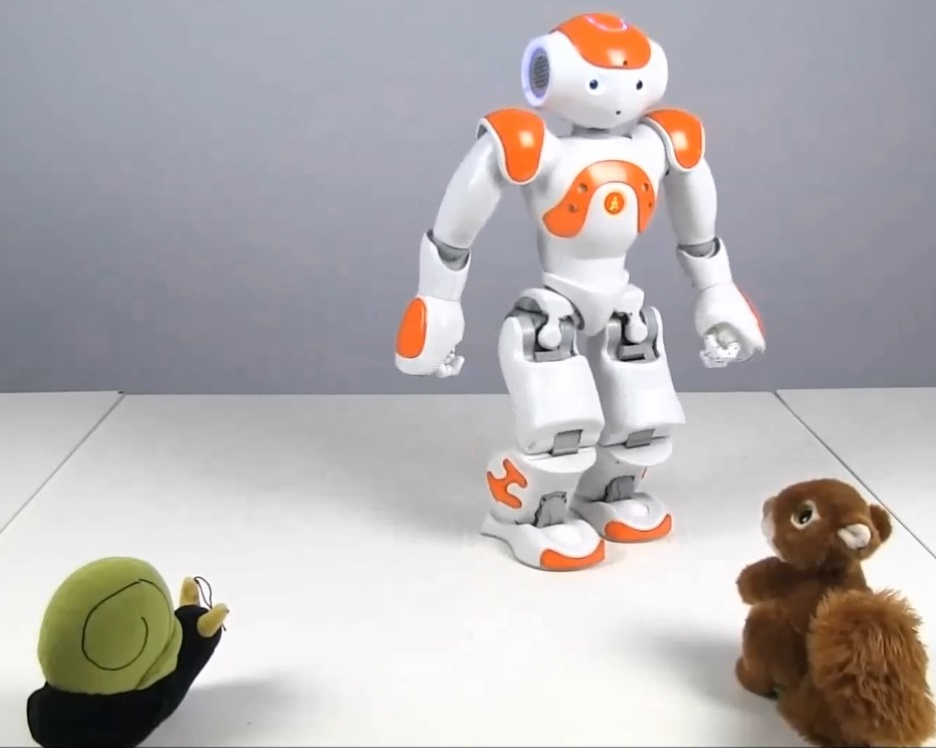
\includegraphics[width=0.5\linewidth]{stimulus-toys}
        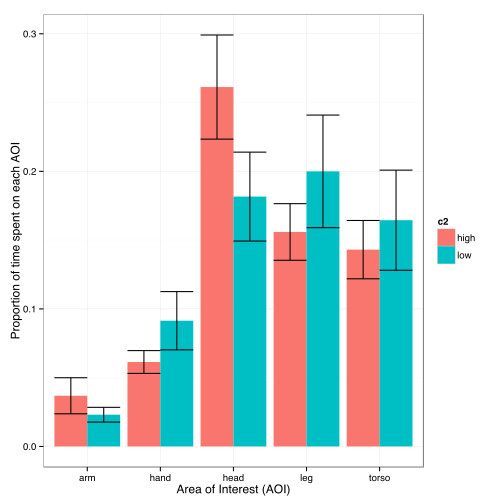
\includegraphics[width=0.5\linewidth]{cognitive-priming}
    \end{center}
\end{frame}
}

%%%%%%%%%%%%%%%%%%%%%%%%%%%%%%%%%%%%%%%%%%%%%%%%%%%%%%%%%%%%%%%%%%%%%%%%%%%%%%%%%
\subsection{With-me-ness}


\imageframe[color=black]{realSetup}
\imageframe{experimental_setup}
\imageframe[color=black]{head_pose_real_world}

{
\paper{Lemaignan et al. {\Medium From Real-time Attention Assessment to “With-me-ness” in Human-Robot Interaction} -- HRI 2016}
\fullbackground[scale=0.95]{with-me-ness-robot}

\begin{frame}{With-me-ness}
\end{frame}
}

{
\paper{Lemaignan, Fink, Dillenbourg {\Medium You're Doing It Wrong! Studying Unexpected Behaviors in Child-Robot Interaction}, ICSR 2015}
\fullbackground{ranger-background}
\begin{frame}{Anthropomorphism != Engagement}

\begin{figure}
    \hspace*{5cm}\includegraphics[width=0.6\textwidth]{ranger-interactions-vs-qualitative-score}
\end{figure}
\end{frame}
}




%%%%%%%%%%%%%%%%%%%%%%%%%%%%%%%%%%%%%%%%%%%%%%%%%%%%%%%%%%%%%%%%%%%%%%%%%%%%%%%%%
%%%%%%%%%%%%%%%%%%%%%%%%%%%%%%%%%%%%%%%%%%%%%%%%%%%%%%%%%%%%%%%%%%%%%%%%%%%%%%%%%
%%%%%%%%%%%%%%%%%%%%%%%%%%%%%%%%%%%%%%%%%%%%%%%%%%%%%%%%%%%%%%%%%%%%%%%%%%%%%%%%%


\section{Bind Them All}
%%%%%%%%%%%%%%%%%%%%%%%%%%%%%%%%%%%%%%%%%%%%%%%%%%%%%%%%%%%%%%%%%%%%%%%%%%%%%%%%%

\imageframe[color=white]{islands1}
\imageframe[color=white]{islands2}
\imageframe[color=white]{islands3}
\imageframe[color=white]{islands4}

{
\paper{Baxter, Lemaignan, Trafton {\Medium Workshop on Cognitive Architectures for Social HRI} -- HRI 2016}
\begin{frame}{Cognitive Architectures for social HRI}

    \begin{multicols}{2}
        \resizebox{0.7\columnwidth}{!}{%
            \begin{tikzpicture}[
                    >=latex,
                every edge/.style={<-, draw, very thick}]

            \path[small mindmap, 
                level 1 concept/.append style={sibling angle=360/6}, 
                level 2 concept/.append style={sibling angle=60}, 
            concept color=hriSec1,text=white]
            node[concept] {Cognitive Architectures}
                [clockwise from=60]
                child[concept color=hriSec3Dark,text=white] { node[concept]{1. Model} }
                child[concept color=hriSec2Dark,text=white] { node[concept]{2. Integration} }
                child[concept color=hriSec2CompDark,text=white] { node[concept] {3. Methodology}};


        \end{tikzpicture}
    }
    \vfill
    \columnbreak

    {\Medium 1. Models of Human Cognition}

    {\scriptsize -- Modelling (aspects of) human cognition \\-- Subsequent application to robots}

    {\Medium 2. Technical Integration}

    {\scriptsize -- Define required functionality of robots \\-- Implement algorithms (etc) necessary}

    {\Medium 3. A Methodology}

    {\scriptsize -- Formalising assumptions \\-- Integrating knowledge from multiple disciplines \\-- Iteratively updating architecture}

    %\refToContrib{Someone here...}

    \end{multicols}
\end{frame}
}


%\imageframe{pr2-baby-4.jpg}
%\imageframe[\scriptsize \Medium Mix of geometry, time, semantics\\ \vspace*{1em}
%        High geometric/temporal granularity (e.g. nodding)\\ \vspace*{1em}
%        Lots of common-sense knowledge, cultural background\\ \vspace*{1em}
%        %Non-monotonic topology\\
%        %Represent continuous/discrete fields\\
%        Account for uncertainties\\ \vspace*{1em}
%        Remember the past, imagine the future\\ \vspace*{1em}
%        %Imagine entities\\
%        %Temporal template matching, chronicles\\
% ]{pr2-baby-4.jpg}
%
%\imageframe[\scriptsize Mix of geometry, time, semantics\\ \vspace*{1em}
%        High geometric/temporal granularity (e.g. nodding)\\ \vspace*{1em}
%        Lots of common-sense knowledge, cultural background\\ \vspace*{1em}
%        %Non-monotonic topology\\
%        %Represent continuous/discrete fields\\
%        Account for uncertainties\\ \vspace*{1em}
%        Remember the past, imagine the future\\ \vspace*{1em}
%        {\Medium
%        Imagine entities {\Light (pre-supposition accomodation)}\\ \vspace*{1em}
%        The world is non-monotonic\\ \vspace*{1em}
%        ...and full of exceptions {\Light (damn pinguins!)}\\ \vspace*{1em}
%        ...
%        }
%        %Temporal template matching, chronicles\\
% ]{pr2-baby-4.jpg}


{
%\fullbackground{background.pdf}
%\begin{frame}[plain]
%
%    Mutual Modelling: from visual perspective taking
%    to...
%\end{frame}
%}

\subsection{A Cognitive Architecture}
{
    \paper{Lemaignan et al., {\Medium Human-Robot Interaction: Tackling AI challenges}, Artifical Intelligence, (hopefully) 2016}
\begin{frame}{From ``Technical Integration''...}
    \begin{figure}
        \centering

        \resizebox{0.9\paperwidth}{!}{%

            \tikzset{subpart/.style={draw, font=\scriptsize, fill opacity=0.5, text opacity=1, fill=white!50}}

            \begin{tikzpicture}[
                    >=latex,
                    every edge/.style={draw, very thick},
                    skill/.style={draw, rounded corners, align=center, inner sep=5pt, fill=black!20},
                label/.style={midway, align=center, font=\scriptsize, fill=white}]

                %%% Separation between deliberative layer and sensori-motor layer
                \draw[dotted, thick] (-8,-5) -- (12, -5);

                %%% SPARK
                \uncover<2->{
                \node at (4,-3.5)[skill, fill=hriSec3!50] (spark) {%
                    \begin{tikzpicture}
                        \node at (0,0) (geom) {Geometric \& Temporal Reasoning -- {\tt spark}};
                        \node [subpart, below=0.2 of geom.south west, anchor=north west] (world-update) {Sensors fusion};
                        \node [subpart, right=0.2 of world-update] (geom-model) {Geometric model of the environment};
                        \node [subpart, right=0.2 of geom-model] (fact-prod) {Symbolic facts production};
                    \end{tikzpicture}
                };
                }

                %%% LOWLEVEL
                \node [skill, below=0.7 of spark] (lowlevel) {%
                    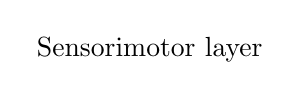
\begin{tikzpicture}
                        \node at (0,0) (sensori) {Sensorimotor layer};
                        %\node [subpart, below=0.2 of sensori.south west, anchor=north west, align=left] (perception) {{\bf Perception} \\ 2D markers, RGB-D, motion capture};
                        %\node [subpart, align=right, right=0.2 of perception] {{\bf Actuation} \\ Head's pan-tilt unit, grippers, arms, wheels};
                    \end{tikzpicture}
                };

                \uncover<2->{
                \path (lowlevel) edge [->] (spark);
                }

                %%% ORO
                \uncover<3->{
                \node at (0,0)[skill, ultra thick, fill=hriSec2Dark!50] (oro)
                {Symbolic facts \\ and beliefs management -- {\tt oro}};
                \path (spark.100) edge [->, bend right] node[label] {symbolic \\ facts} (oro);
                }

                %%% HATP
                \uncover<5->{
                \node at (-6, 2.5)[skill, fill=hriSec1!50] (hatp) {Human-aware
                symbolic \\task planning -- {\tt hatp}};
                \path (hatp) edge [<->, bend right] node[label] {world model and \\ agents beliefs} (oro.170);
                }

                %%% DIALOGS
                \uncover<4->{
                \node at (-6, -3) [skill, fill=hriSec3Dark!50] (dialogs)
                {Dialogue processing\\{\tt dialogs}};
                \path (dialogs) edge [<->, bend left] node[label] {natural language \\ grounding} (oro.190);
                }
                %%% SHARY
                \uncover<5->{
                \node at (4,4.5)[skill, fill=hriSec1Comp!50] (shary) {%
                    \begin{tikzpicture}
                        \node at (0,0) (exec) {Execution Controller -- {\tt shary} | {\tt pyrobots}};
                        \node [subpart, below=0.2 of exec.south west, anchor=north west] (plans) {Goal \& Plans \\ management};
                        \node [subpart, right=0.2 of plans] (sit-asses) {Situation assessment \\ and context management};
                        \node [subpart, right=0.2 of sit-asses] {Action instantiation, \\ execution and monitoring};
                    \end{tikzpicture}
                };
                \path (shary) edge [<->, bend left] node[label] {events, \\ world model and \\ agents beliefs} (oro);
                \path (shary) edge [<->, bend left, looseness=0.8] node[label] {action monitoring \\ and management of \\ position hypotheses} (spark);
                \path (shary.west) edge [<->, bend right] node[label] {shared \\ plans} (hatp);
                }
                %%% MHP
                \uncover<6->{
                \node at (9,0)[skill, fill=hriSec3CompDark!50] (mhp) {Human-aware Motion \\ and Manipulation Planning\\{\tt mhp}};
                \path (shary.340) edge [<->, bend left] node[label] {motion plan \\ requests} (mhp);
                \path (spark.5) edge [->, bend right] node[label] {environment\\model} (mhp);
                \path (lowlevel.east) edge [<-, bend right=60, looseness=1.3] node[label] {atomic\\actions} (mhp.south east);
                }



            \end{tikzpicture}
        }
    \end{figure}

\end{frame}
}


{

    \paper{Devin et al. {\Medium Some essential skills and their combination in an architecture for a cognitive and interactive robot} -- HRI 2016}
\begin{frame}{...to ``Modeling of human cognition''...}

\resizebox{!}{0.7\paperheight}{%
\tikzset{subpart/.style={draw, font=\scriptsize, fill opacity=0.5, text opacity=1, fill=white!50}}
\begin{tikzpicture}[
    >=latex,
    node distance=1.5,
    every edge/.style={draw, very thick},
    skill/.style={draw, rounded corners, align=center, inner sep=5pt, fill=black!20},
    stmt/.style={align=center, font=\Medium},
    label/.style={midway, align=center, font=\scriptsize, fill=white}]

    \node at (0,0)[skill, fill=hriSec2!50] (a1) {Shared Plan Elaboration};

    \node [skill, fill=hriSec2!50,above=of a1] (a2) {Intention Prediction};
    \node [skill, fill=hriSec2!50,left=of a1] (a3) {Mental State Management};
    \node [skill, fill=hriSec2!50,right=of a1] (a4) {Communication for\\Joint Action};
    \node [skill, fill=hriSec2!50,below=of a1] (a5) {Shared Plan Achievement};
    \node [skill, fill=hriSec2!50,left=of a5] (a6) {Situation Assessment};


    \node [skill, fill=hriSec3!50,below left=of a5,anchor=north] (a7) {Action Achievement};
    \node [skill, fill=hriSec3!50,below right=of a5,anchor=north] (a8) {Human Action Monitoring};
  
    \node[below=3.7 of a5] (a14) {Human-aware geometric and task planners, real-time controllers, sensors...};

  \coordinate[below=3 of a6] (a9);

  \node[rotate=90,left=0.7 of a3.west] (distal) {\Medium\large DISTAL};
  \node[rotate=90] at (distal |- a7.south) {\Medium\large PROXIMAL};
  \node[rotate=90] at (distal |- a14) {\Medium\large MOTOR};

  \coordinate (a11) at (a9 -| distal.north);
  \coordinate (a12) at (a9 -| a4.east);
  \draw[dotted, thick] (a11) -- (a12);


  \coordinate (a13) at ($(a5)!0.5!(a7)$);
  \draw[dotted, thick] (a13 -| distal.north) -- (a13 -| a4.east);


  %%% Relations between components
  \path (a2) edge [->] node[label] {goal to execute} (a1);
  \path (a1) edge [->] node[label] {plan} (a5);
  \path (a2) edge [<-] node[label] {goal (order)} (a4);

  \path (a3) edge [<->, bend left=40, looseness=1.2] node[label,pos=0.1] {mental state information} (a4);
  \path (a3) edge [<->] (a2);
  \path (a3) edge [<->] (a1);
  \path (a3) edge [<->] (a5);

  \path (a6) edge [->] node[label] {conceptual\\world state} (a3);

  \path (a5) edge [<->] node[label] {coordination} (a4);

  \path (a5) edge [<->] node[label,right=0.5] {anchoring of actions} (a7);
  \path (a5) edge [<->] (a8);

  \path (a9) edge [->] node[label] {sensors} (a6);

  \coordinate (a10) at (a9 -| a7);
  \path (a10) edge [<->] node[label] {planning and control} (a7);

  \coordinate (a10) at (a9 -| a8);
  \path (a10) edge [<->] node[label] {sensors} (a8);

  \path (a7) edge [<->] node[label] {coordination} (a8);
 
\end{tikzpicture}
}

\end{frame}
}
%%%%%%%%%%%%%%%%%%%%%%%%%%%%%%%%%%%%%%%%%%%%%%%%%%%%%%%%%%%%%%%%%%%%%%%%%%%%%%%%%
%%%%%%%%%%%%%%%%%%%%%%%%%%%%%%%%%%%%%%%%%%%%%%%%%%%%%%%%%%%%%%%%%%%%%%%%%%%%%%%%%
%%%%%%%%%%%%%%%%%%%%%%%%%%%%%%%%%%%%%%%%%%%%%%%%%%%%%%%%%%%%%%%%%%%%%%%%%%%%%%%%%


\section{A Summary and Some Ideas}
%%%%%%%%%%%%%%%%%%%%%%%%%%%%%%%%%%%%%%%%%%%%%%%%%%%%%%%%%%%%%%%%%%%%%%%%%%%%%%%%%

\begin{frame}{The Experimental Summary}

    \begin{multicols}{4}
        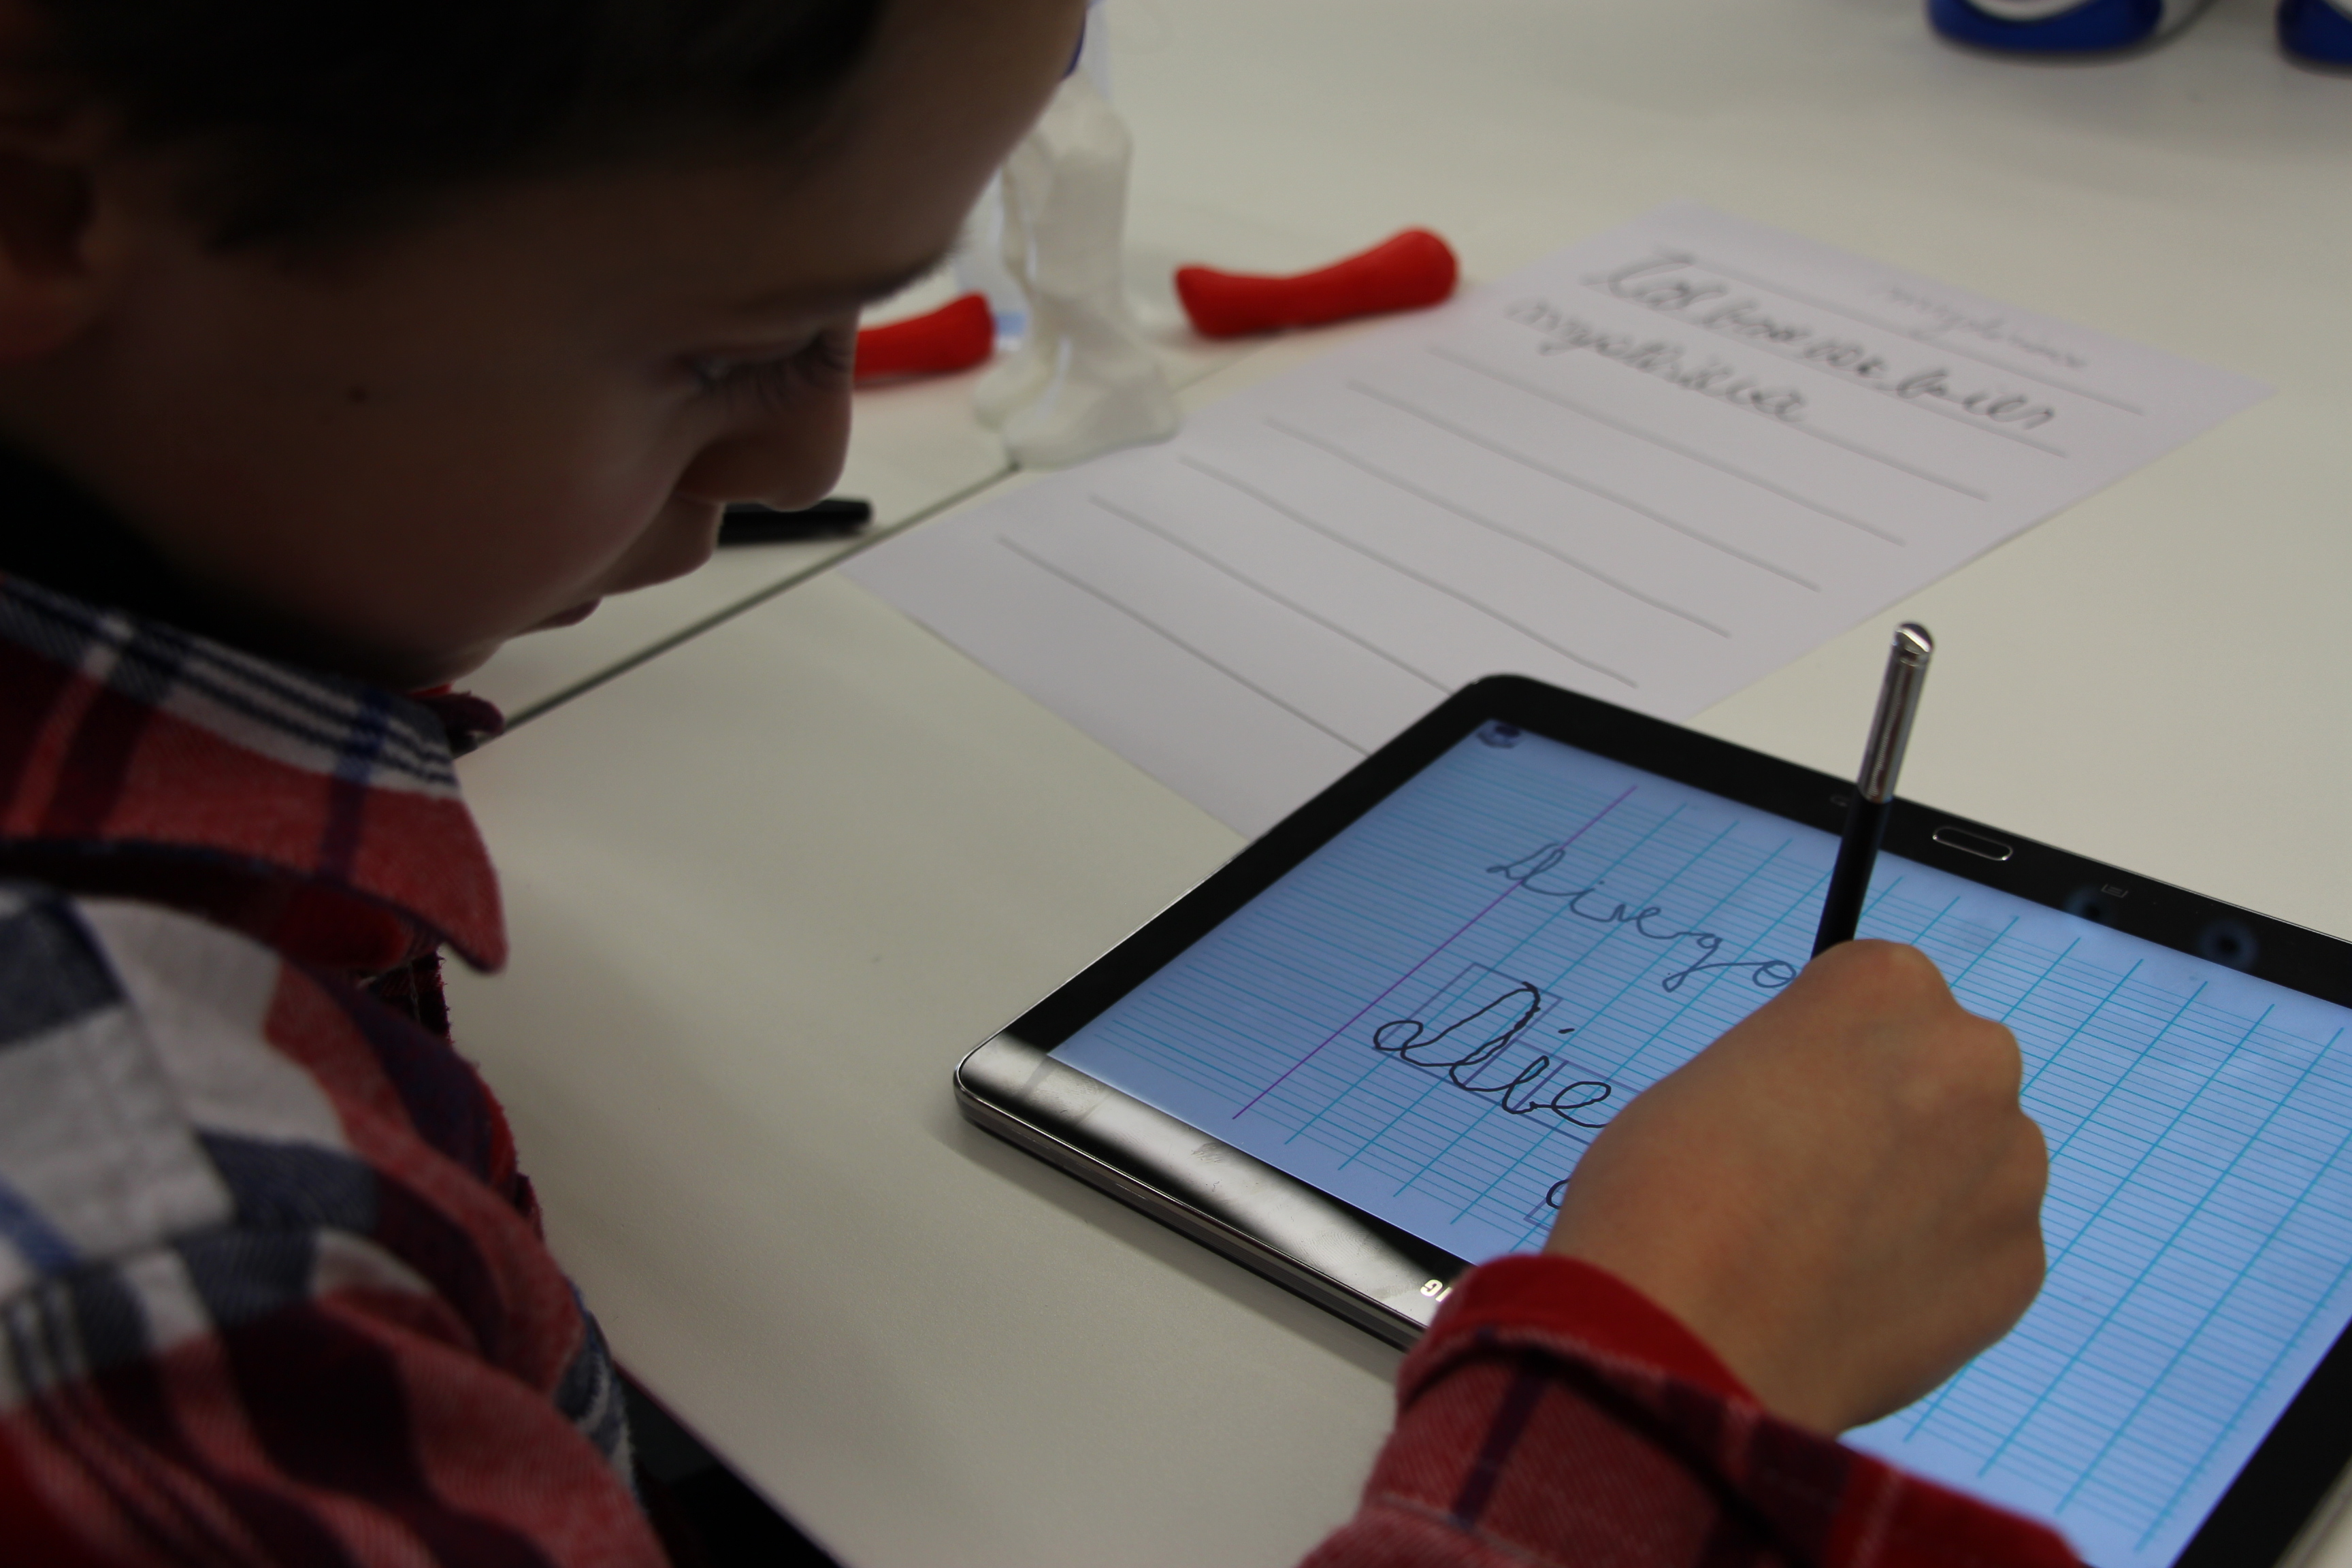
\includegraphics[width=\columnwidth]{diego-writing}

        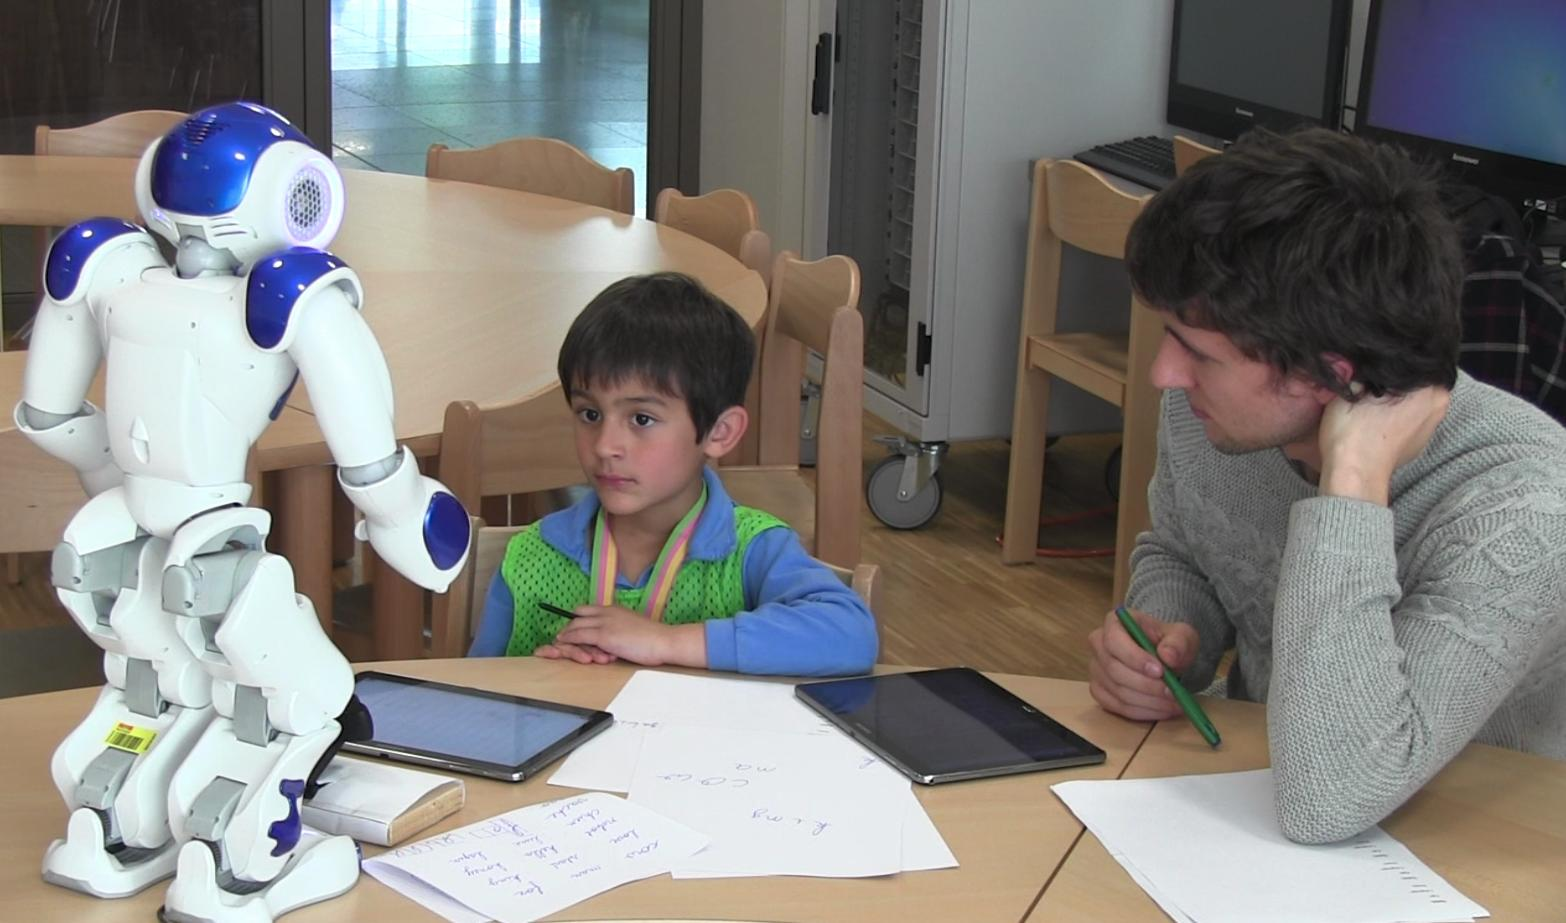
\includegraphics[width=\columnwidth]{realSetup}

        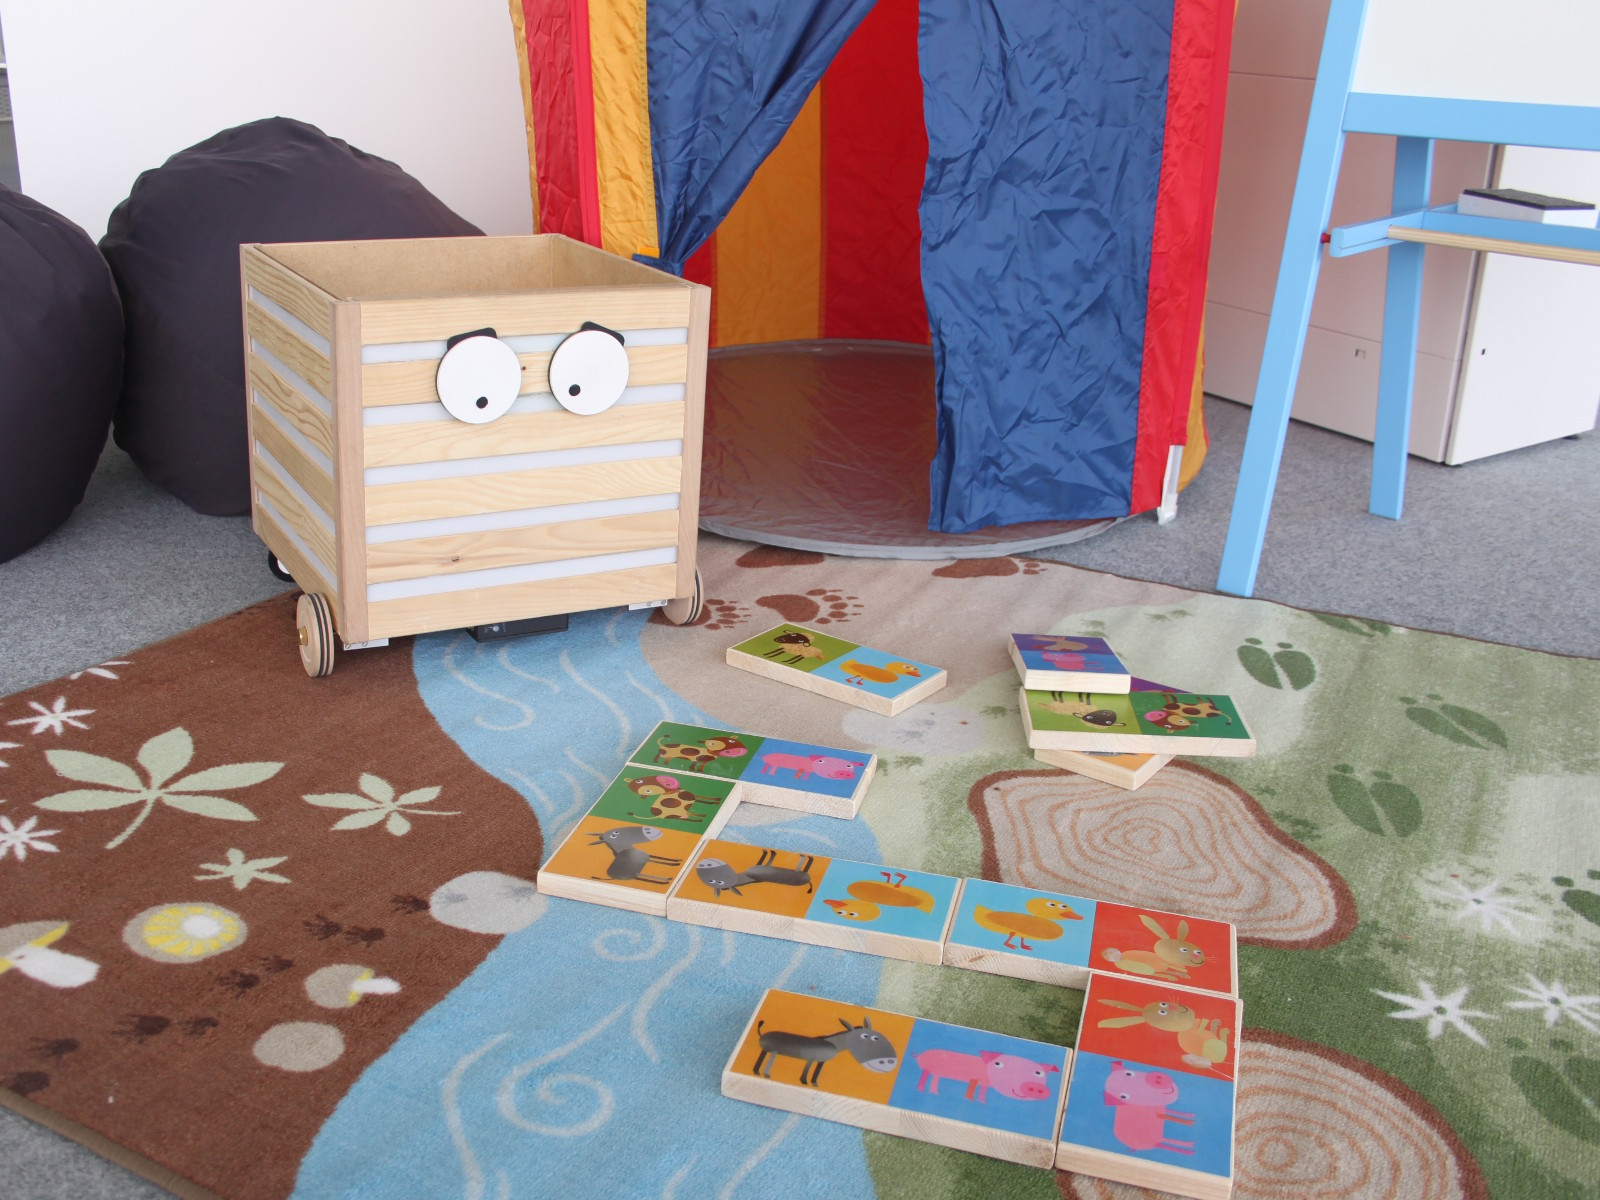
\includegraphics[width=\columnwidth]{ranger-background}

        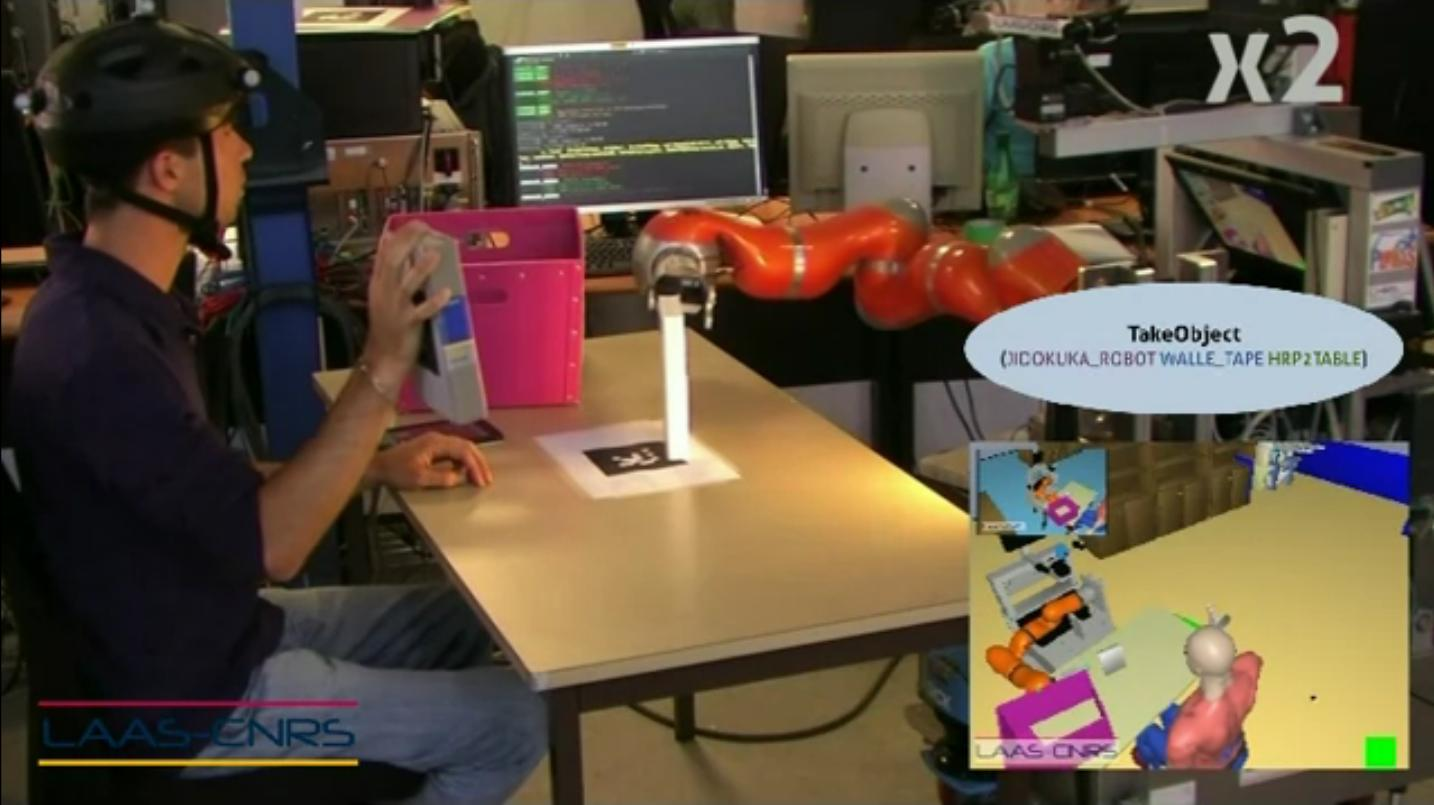
\includegraphics[width=\columnwidth]{cleantable}

        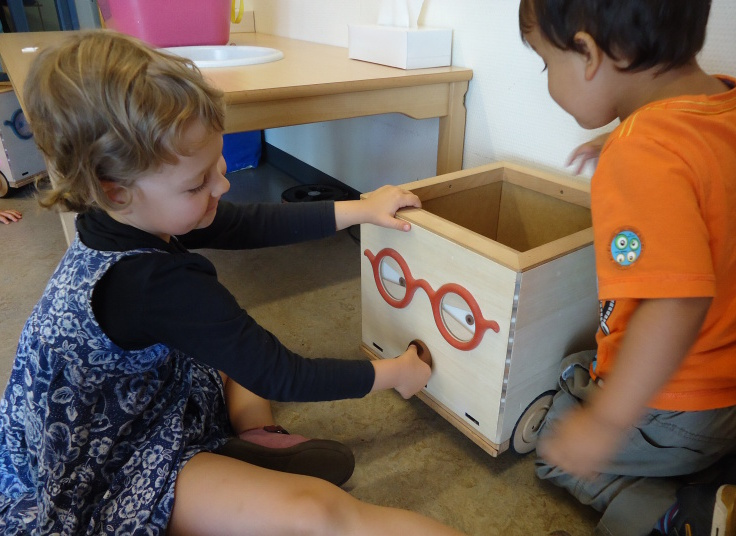
\includegraphics[width=\columnwidth]{croquignole-single}

        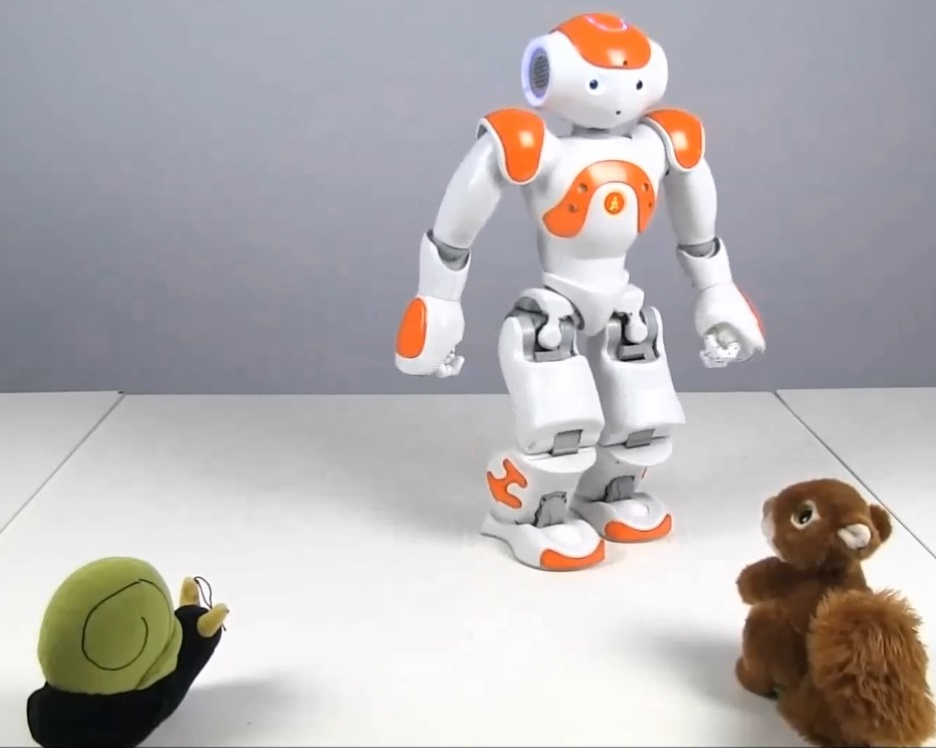
\includegraphics[width=\columnwidth]{stimulus-toys}

        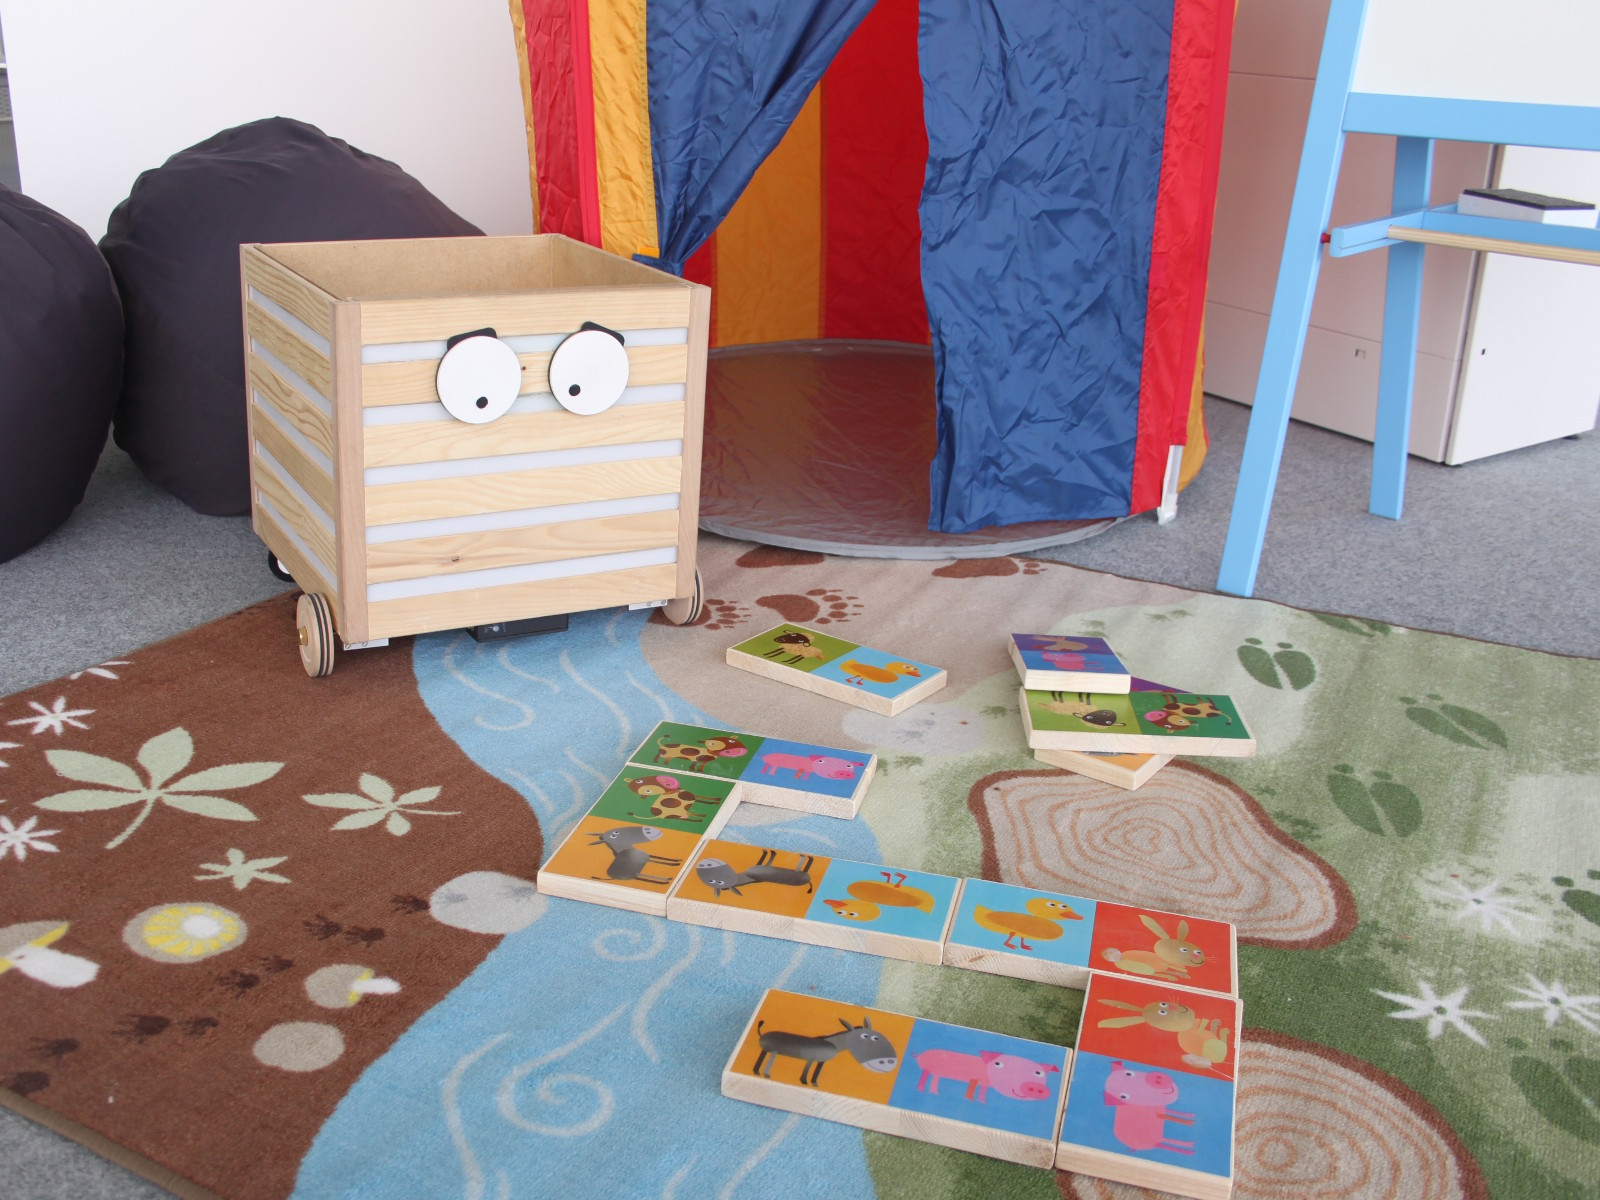
\includegraphics[width=\columnwidth]{ranger-background}

        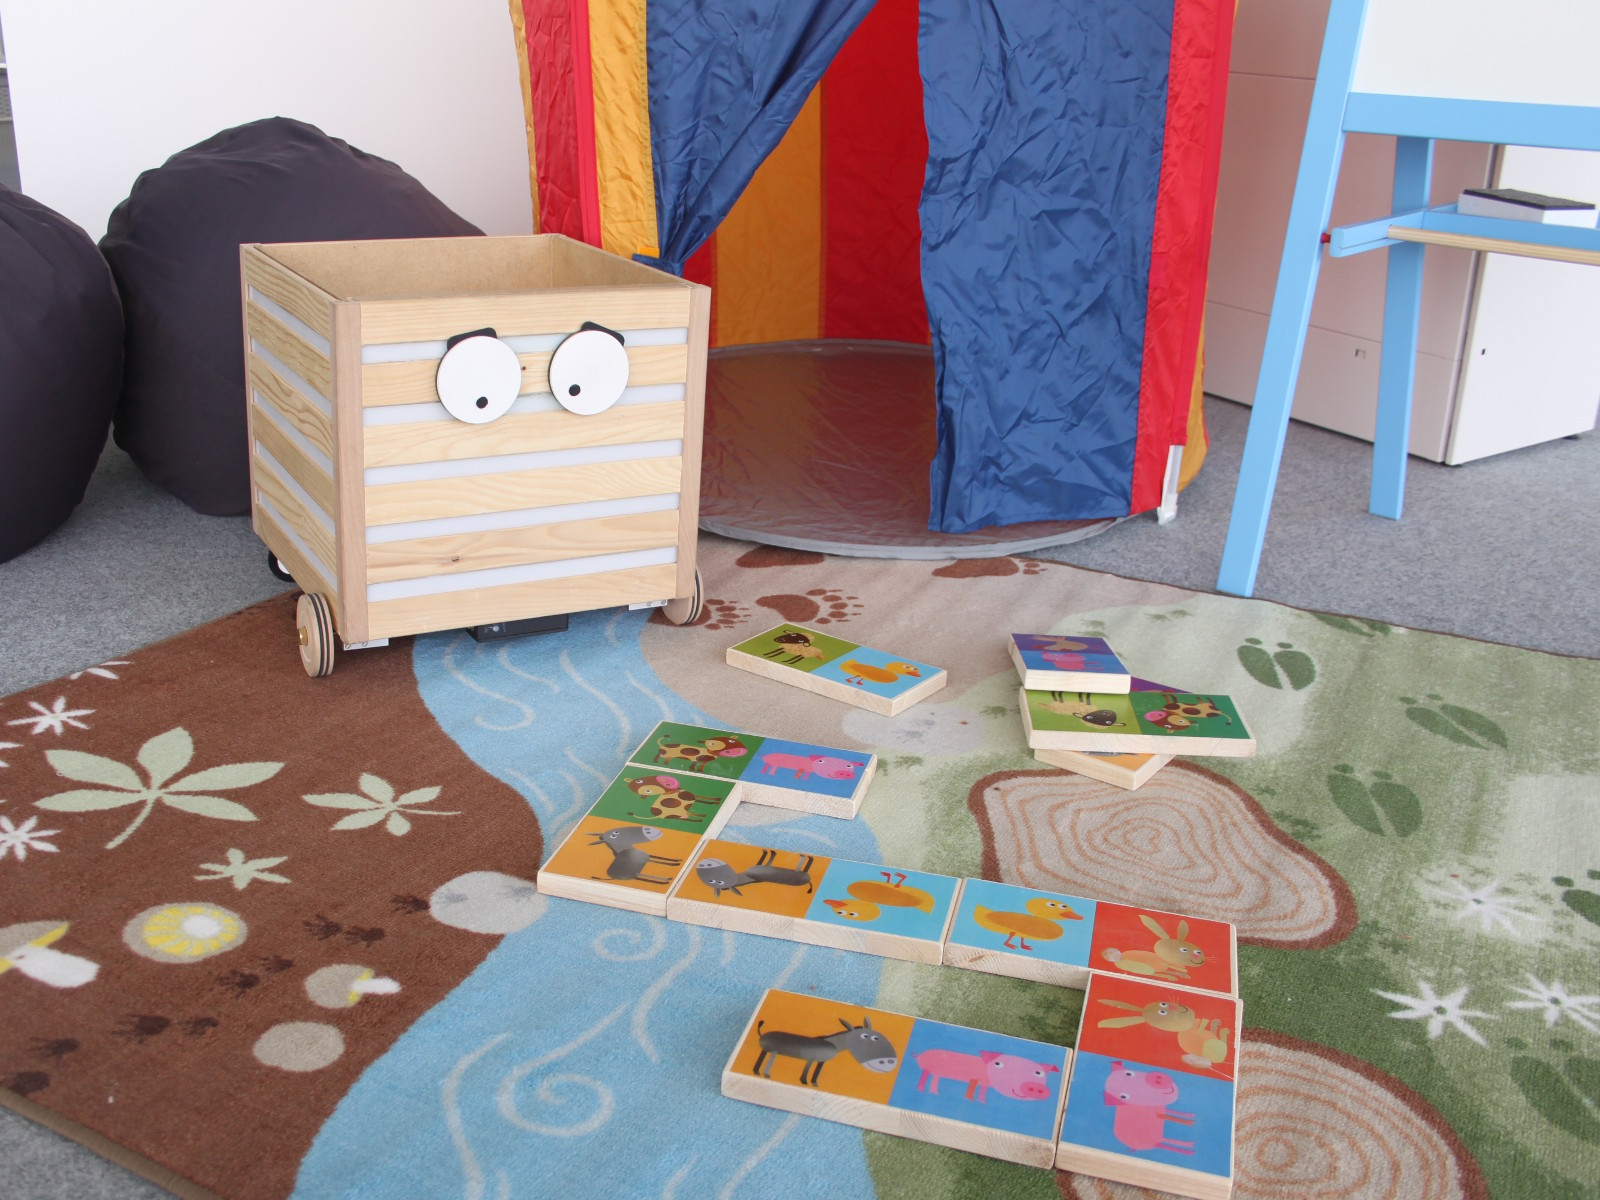
\includegraphics[width=\columnwidth]{ranger-background}

        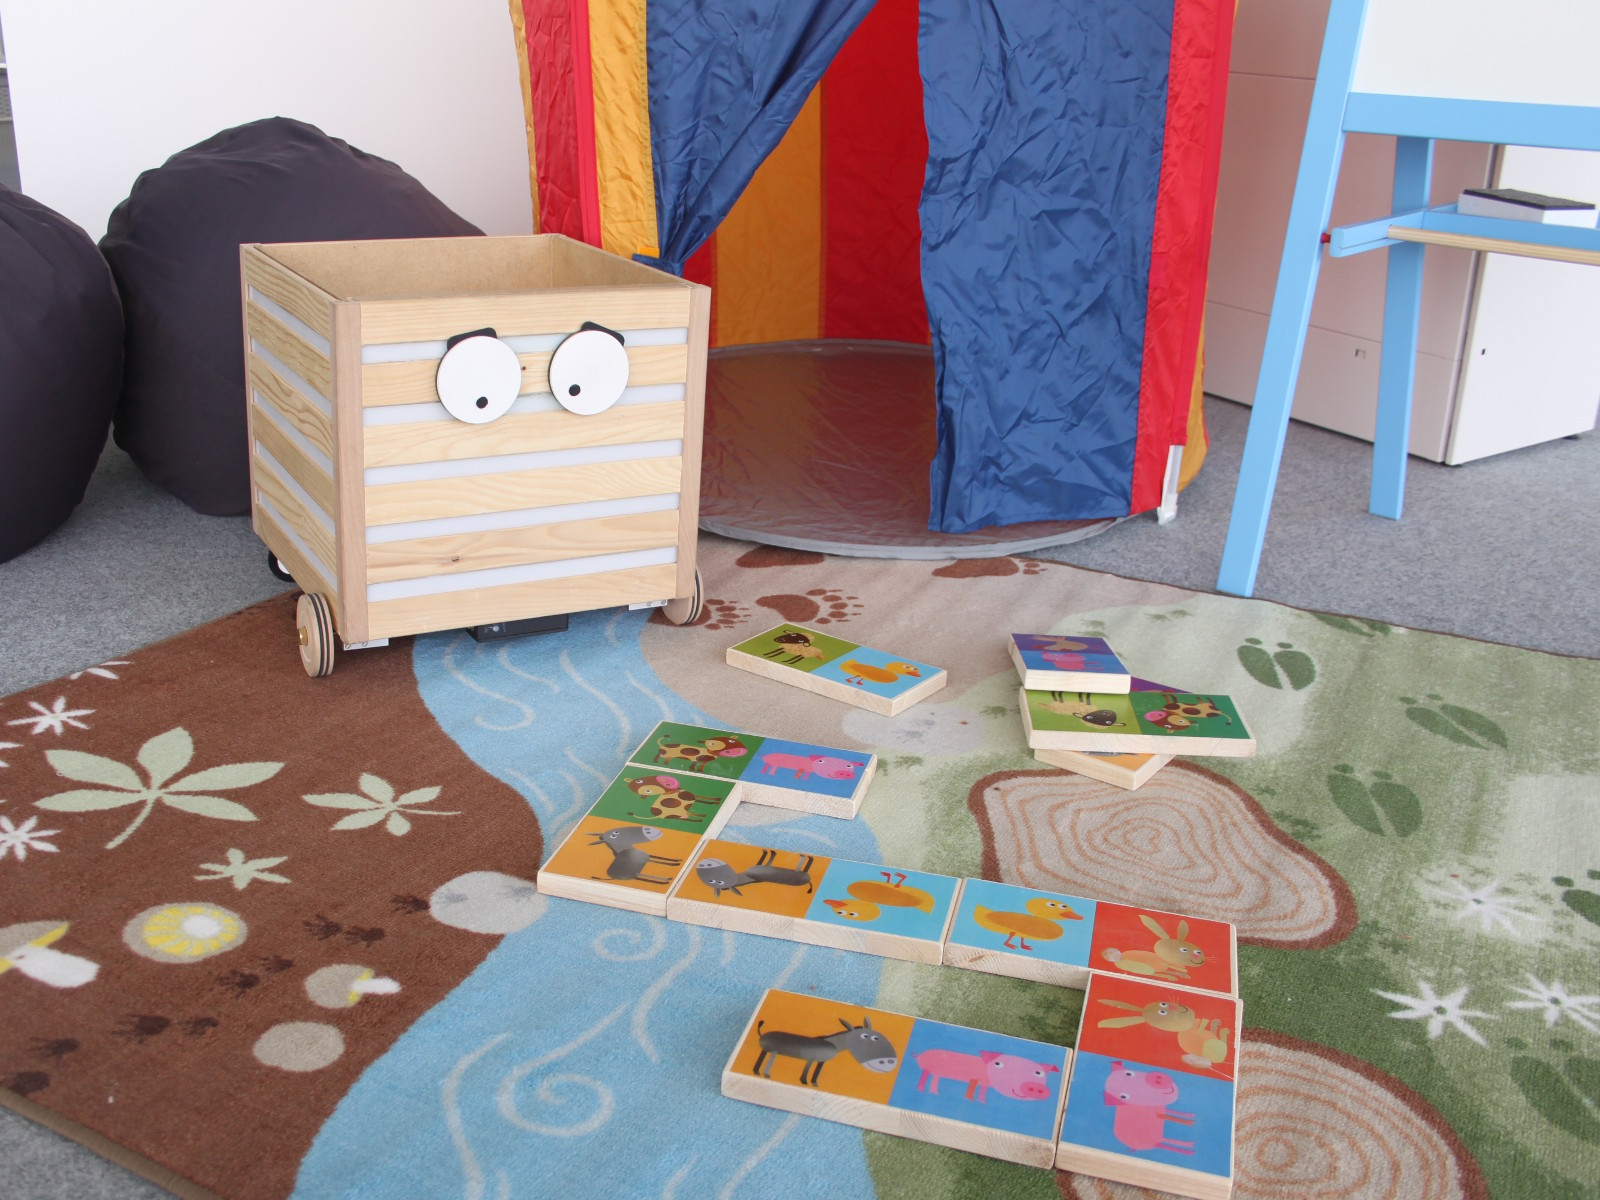
\includegraphics[width=\columnwidth]{ranger-background}
    \end{multicols}


\end{frame}

{
    \paper{Mnih et al. {\Medium Human-level control through deep reinforcement learning} -- Nature 2015}
\begin{frame}{Learning Complex Behaviours}

    \begin{center}
        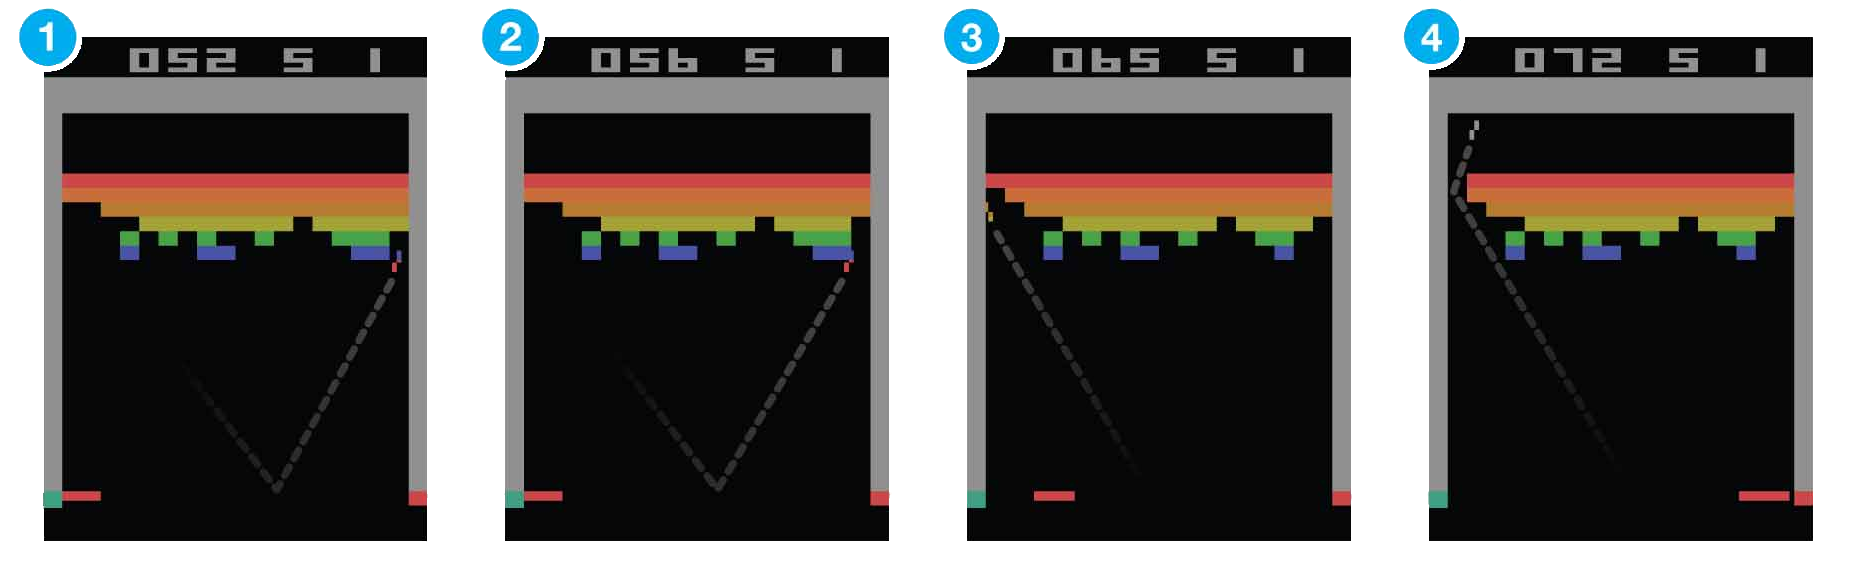
\includegraphics[width=\linewidth]{breakout}
    \end{center}


        \begin{itemize}
            \item Inputs: raw screen image + score
            \item from the outside, looks like planning
            \item<2-> \sout{1.000.000} {\Medium 500} games to play a good human-level
        \end{itemize}

    \uncover<3> {
        \begin{center}
            {\Medium Could we also learn social dynamics?}
        \end{center}
    }
\end{frame}
}


\begin{frame}{Attention, Alignment, Awareness}

    \begin{center}
        \includegraphics<1>[height=0.7\pageheight]{playing_together}
        \includegraphics<2>[height=0.7\pageheight]{playing_together_gaze}
        \includegraphics<3>[height=0.7\pageheight]{playing_together_awareness}
        \includegraphics<4>[height=0.7\pageheight]{playing_together_mutual_awareness}
    \end{center}
\end{frame}


{
    \paper{Baxter et al. {\Medium Cognitive Architecture for HRI: Towards Behavioural Alignment} -- 2013}
\begin{frame}{Associative Memory}

    \centering
        \resizebox{0.8\linewidth}{!}{%
            \begin{tikzpicture}[
                    >=latex,
                every edge/.style={draw, very thick},
                every node/.style={font=\Medium,align=center},
                input/.style={draw,circle, inner sep=0pt,minimum size=0.6cm}
            ]

            % draw the units
                \foreach \x [count=\xi] in {0, 120, 240}
                \foreach \y [count=\yi] in {-.6, 0, .6}
                %\node[input, ball color=orange!\x!blue] at ($(\x:3)!\y!90:(0,0)$) (i\xi\yi) {};
                    \node[input, fill=hriSec3Comp!\x!hriSec1Comp] at ($(\x:3)!\y!90:(0,0)$) (i\xi\yi) {};

                \node[draw,rounded corners, fit=(i11)(i12)(i13)] (modA) {};
                \node[draw,rounded corners, rotate fit=120,fit=(i21)(i22)(i23)] (modB) {};
                \node[draw,rounded corners, rotate fit=60,fit=(i31)(i32)(i33)] (modC) {};

                \uncover<1>{
                    \node at (180:5.5) {Modalities} edge[->] (modB) edge[->] (modC);
                \node at (-40:6) {Input\\units} edge[->] (i13) edge[->] (i31);
                \node at (1,1) {Associative\\links};
            }

                \uncover<2>{
                    \node[above=0.3 of i21]{Bert};
                \node[above=0.3 of i22]{Tony};
                \node[above=0.3 of i23]{Chris};

                \node[right=0.3 of i11]{Green cube in focus};
                \node[right=0.3 of i12]{Red cube in focus};
                \node[right=0.3 of i13]{Board in focus};
            }

                \path[draw,dashed, hriSec3Dark, thick]  (i23) -- (i11) -- (i31) -- (i23);
                \path[draw,dotted, hriSec3Dark, thick] (i23) -- (i12) -- (i32) -- (i23);
                \path[draw, hriSec3Dark] (i21) -- (i13) -- (i33) -- (i21);

            \end{tikzpicture}
    }


\end{frame}
}

%%%%%%%%%%%%%%%%%%%%%%%%%%%%%%%%%%%%%%%%%%%%%%%%%%%%%%%%%%%%%%%%%%%%%%%%%%%%%%%%%
%%%%%%%%%%%%%%%%%%%%%%%%%%%%%%%%%%%%%%%%%%%%%%%%%%%%%%%%%%%%%%%%%%%%%%%%%%%%%%%%%
%%%%%%%%%%%%%%%%%%%%%%%%%%%%%%%%%%%%%%%%%%%%%%%%%%%%%%%%%%%%%%%%%%%%%%%%%%%%%%%%%
%%%%                          THE END                                        %%%%
%%%%%%%%%%%%%%%%%%%%%%%%%%%%%%%%%%%%%%%%%%%%%%%%%%%%%%%%%%%%%%%%%%%%%%%%%%%%%%%%%
%%%%%%%%%%%%%%%%%%%%%%%%%%%%%%%%%%%%%%%%%%%%%%%%%%%%%%%%%%%%%%%%%%%%%%%%%%%%%%%%%
%%%%%%%%%%%%%%%%%%%%%%%%%%%%%%%%%%%%%%%%%%%%%%%%%%%%%%%%%%%%%%%%%%%%%%%%%%%%%%%%%

{
\fullbackground{collage}
\begin{frame}[plain]{}

    {\Medium Thank you!}

    {\Medium\tt\scriptsize severin.lemaignan@plymouth.ac.uk}

    \vfill
        \resizebox{!}{0.6\paperheight}{%
            \begin{tikzpicture}[
                    >=latex,
                every edge/.style={<-, draw, very thick}]
        

            \path[small mindmap, 
                level 1 concept/.append style={sibling angle=360/6}, 
                level 2 concept/.append style={sibling angle=60}, 
            concept color=white,text=hriWarmGreyDark]
            node[concept] {\Medium Social\\Cognition in HRI}
            [clockwise from=30]
            child[concept color=hriSec1,text=white] { node[concept] (percept) {Perception of Human's State}
                [clockwise from=120]
                child[concept color=hriSec3Dark,text=white] { node[concept]{Emotions} }
                child[concept color=hriSec2Dark,text=white] { node[concept]{Attention} }
                child[concept color=hriSec2CompDark,text=white] { node[concept]
                {Inference of mental models} };
            }
            child[concept color=hriSec2Comp,text=white,grow=-30] { node[concept] (knowledge) {Social Knowledge} 
                [counterclockwise from=-120]
                child[concept color=hriSec1CompDark,text=white] { node[concept] {Social rules} }
                child[concept color=hriSec3Comp,text=black] { node[concept] {Social context} }
                child[concept color=hriSec3CompDark,text=white] { node[concept]
                {Common-sense} };
            }
            child[concept color=hriSec3Comp,text=black, grow=-120] { node[concept] (comm) {Communication} 
                [counterclockwise from=180]
                child[concept color=hriSec1CompDark,text=white] { node[concept] {Verbal} }
                child[concept color=hriSec1Dark,text=white] { node[concept]
                {Non-verbal} };
            }
            child[concept color=hriSec3,text=white,grow=180] { node[concept] (dynamics) {Interaction Dynamics} 
                [clockwise from=180]
                child[concept color=hriSec2Dark,text=white] { node[concept]
                {Long-term interaction} };
            }
            child[concept color=hriSec2,text=black, grow=120] { node[concept]
                (action) {Performing with humans} 
                [counterclockwise from=80]
                child[concept color=hriSec2CompDark,text=white] { node[concept] {Action, behaviour recognition} }
                child[concept color=hriSec1Dark,text=white] { node[concept] {Intention reading} }
                child[concept color=hriSec3,text=white] { node[concept] {Joint
                actions} };
            };

        \end{tikzpicture}

    }

\end{frame}
}



%%%%%%%%%%%%%%%%%%%%%%%%%%%%%%%%%%%%%%%%%%%%%%%%%%%%%%%%%%%%%%%%%%%%%%%%%%%%%%%%%
%%%%%%%%%%%%%%%%%%%%%%%%%%%%%%%%%%%%%%%%%%%%%%%%%%%%%%%%%%%%%%%%%%%%%%%%%%%%%%%%%
%%%%%%%%%%%%%%%%%%%%%%%%%%%%%%%%%%%%%%%%%%%%%%%%%%%%%%%%%%%%%%%%%%%%%%%%%%%%%%%%%
%%%%                SUPPLEMENTARY MATERIAL                                   %%%%
%%%%%%%%%%%%%%%%%%%%%%%%%%%%%%%%%%%%%%%%%%%%%%%%%%%%%%%%%%%%%%%%%%%%%%%%%%%%%%%%%
%%%%%%%%%%%%%%%%%%%%%%%%%%%%%%%%%%%%%%%%%%%%%%%%%%%%%%%%%%%%%%%%%%%%%%%%%%%%%%%%%
%%%%%%%%%%%%%%%%%%%%%%%%%%%%%%%%%%%%%%%%%%%%%%%%%%%%%%%%%%%%%%%%%%%%%%%%%%%%%%%%%



\imageframe[caption="Theory of Mind tasks"]{zoo}

\begin{frame}{Unexpected behaviours}

    \centering
    \begin{tabular}{  >{\centering\arraybackslash}m{2cm} | >{\centering\arraybackslash}m{2cm} | >{\centering\arraybackslash}m{2cm} }
        & Unplanned by the robot & Planned by the robot \\ \hline
        Perceived as non-intentional & A  & B  \\ \hline
        Perceived as intentional &  C & D 
    \end{tabular}

    \video{0.4\paperwidth}{videos/ranger-correct.m4v}
    \video{0.4\paperwidth}{videos/ranger-disobey.m4v}

\end{frame}


%%%%%%%%%%%%%%%%%%%%%%%%%%%%%%%%%%%%%%%%%%%%%%%%%%%%%%%%%%%%%%%%%%%%%%%%%%%%%%%
%\subsection{CoWriter}

\begin{frame}{CoWriter details}
    \centering
    CoWriter: Learning by Teaching\\

    \only<1>{
    \video{0.8\textwidth}{videos/nao-tablet-demo.mp4}
    }

    \only<2>{
        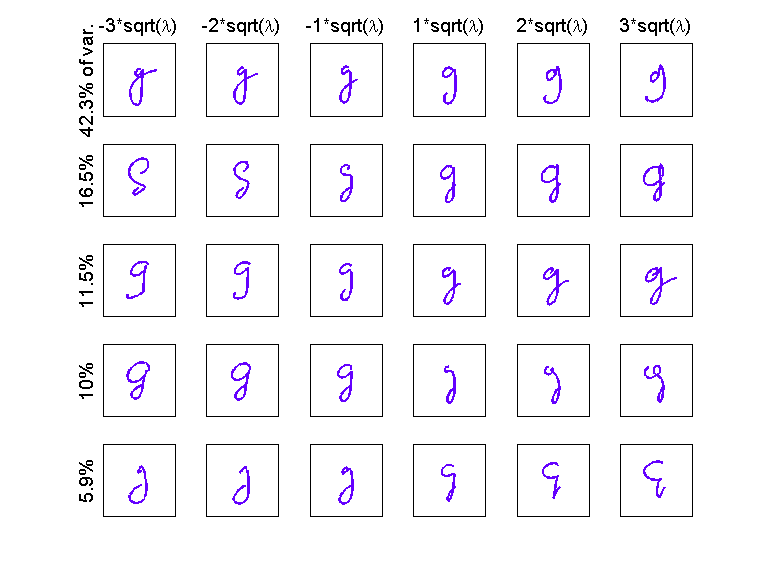
\includegraphics[width=0.8\textwidth]{cowriter-g.png}
    }


    \only<3>{
    \video{0.8\textwidth}{videos/cowriter-session1_3minExcerpt_1x.mp4}
    }

\end{frame}

\imageframe{cowriter-fsm.png}

%%%%%%%%%%%%%%%%%%%%%%%%%%%%%%%%%%%%%%%%%%%%%%%%%%%%%%%%%%%%%%%%%%%%%%%%%%%%%%%
%%%%%%%%%%%%%%%%%%%%%%%%%%%%%%%%%%%%%%%%%%%%%%%%%%%%%%%%%%%%%%%%%%%%%%%%%%%%%%%
%%%%%%%%%%%%%%%%%%%%%%%%%%%%%%%%%%%%%%%%%%%%%%%%%%%%%%%%%%%%%%%%%%%%%%%%%%%%%%%

%\section{Act}

%%%%%%%%%%%%%%%%%%%%%%%%%%%%%%%%%%%%%%%%%%%%%%%%%%%%%%%%%%%%%%%%%%%%%%%%%%%%%%%

%%%%%%%%%%%%%%%%%%%%%%%%%%%%%%%%%%%%%%%%%%%%%%%%%%%%%%%%%%%%%%%%%%%%%%%%%%%%%%%
%\subsection{Planning}


\begin{frame}{Planning for the Human}

    \begin{figure}
        \centering

        \resizebox{0.7\paperwidth}{!}{%
            \begin{tikzpicture}[
                    >=latex,
                    robot/.style={fill=hriSec1CompDark!50},
                    every edge/.style={<-, draw, ultra thick},
                    every node/.style={ draw, 
                        thick,  
                        circle, 
                        font=\sf,
                        align=center,
                        node distance=2cm,
                        fill=hriSec3CompDark!50, 
                        minimum size=2cm, 
                inner sep=0.1cm}]

                \node[font=\large, draw=none, fill=none, rotate=90] at (-2, 0) {Human\\actions};
                \node[font=\large, draw=none, fill=none, rotate=90] at (-2, -3.5) {Robot\\actions};

                \node (h1) {\hatpaction{TAKE}{GREY\_TAPE}{TABLE}};
                \node[right=of h1] (h2) {\hatpaction{PUT}{GREY\_TAPE}{BIN1 }} edge (h1);

                \node[robot, below=1.5 of h1] (r1) {\hatpaction{TAKE}{BLACK\_TAPE}{TABLE }};
                \node[robot, right=of r1] (r2) {\hatpaction{PUT}{BLACK\_TAPE}{BIN2 }} edge (r1);
                \node[robot, right=of r2] (r3) {\hatpaction{TAKE}{BOTTLE}{TABLE }} edge (r2);
                \node[robot, right=of r3] (r4) {\hatpaction{PUTRV}{BOTTLE}{TABLE}} edge (r3);
                \node[robot, right=of r4] (r5) {\hatpaction{TAKE}{BOOK}{TABLE }} edge (r4);
                \node[robot, right=of r5] (r6) {\hatpaction{PUT}{BOOK}{BIN2 }} edge (r5);

                \node at (r5 |- h1) (h3) {\hatpaction{TAKE}{BOTTLE}{TABLE}} edge (h2) edge (r4);
                \node[right=of h3] (h4) {\hatpaction{PUT}{BOTTLE}{BIN1}} edge (h3);

            \end{tikzpicture}
        }

        \vspace*{1cm}

        \onslide<2>
        \resizebox{0.7\paperwidth}{!}{%
            \begin{tikzpicture}[
                    >=latex,
                    robot/.style={fill=hriSec1CompDark!50},
                    every edge/.style={<-, draw, ultra thick},
                    every node/.style={ draw, 
                        thick,  
                        circle, 
                        font=\sf,
                        align=center,
                        node distance=2cm,
                        fill=hriSec3CompDark!50, 
                        minimum size=2cm, 
                inner sep=0.1cm}]

                \node[font=\large, draw=none, fill=none, rotate=90] at (-2, 0) {Human\\actions};
                \node[font=\large, draw=none, fill=none, rotate=90] at (-2, -3.5) {Robot\\actions};


                \node (h1) {\hatpaction{TAKE}{GREY\_TAPE}{TABLE}};
                \node[right=of h1] (h2) {\hatpaction{PUT}{GREY\_TAPE}{BIN1 }} edge (h1);

                \node[robot, below=1.5 of h1] (r3) {\hatpaction{TAKE}{BOTTLE}{TABLE }};
                \node[robot, right=of r3] (r4) {\hatpaction{PUTRV}{BOTTLE}{TABLE}} edge (r3);
                \node[robot, right=of r4] (r1) {\hatpaction{TAKE}{BLACK\_TAPE}{TABLE }} edge (r4);
                \node[robot, right=of r1] (r2) {\hatpaction{PUT}{BLACK\_TAPE}{BIN2 }} edge (r1);
                \node[robot, right=of r2] (r5) {\hatpaction{TAKE}{BOOK}{TABLE }} edge (r2);
                \node[robot, right=of r5] (r6) {\hatpaction{PUT}{BOOK}{BIN2 }} edge (r5);

                \node[right=of h2] (h3) {\hatpaction{TAKE}{BOTTLE}{TABLE}} edge (h2) edge (r4);
                \node[right=of h3] (h4) {\hatpaction{PUT}{BOTTLE}{BIN1}} edge (h3);

            \end{tikzpicture}
        }

    \end{figure}
\end{frame}

\begin{frame}{Planning for the Human}

    \begin{figure}
        \centering
        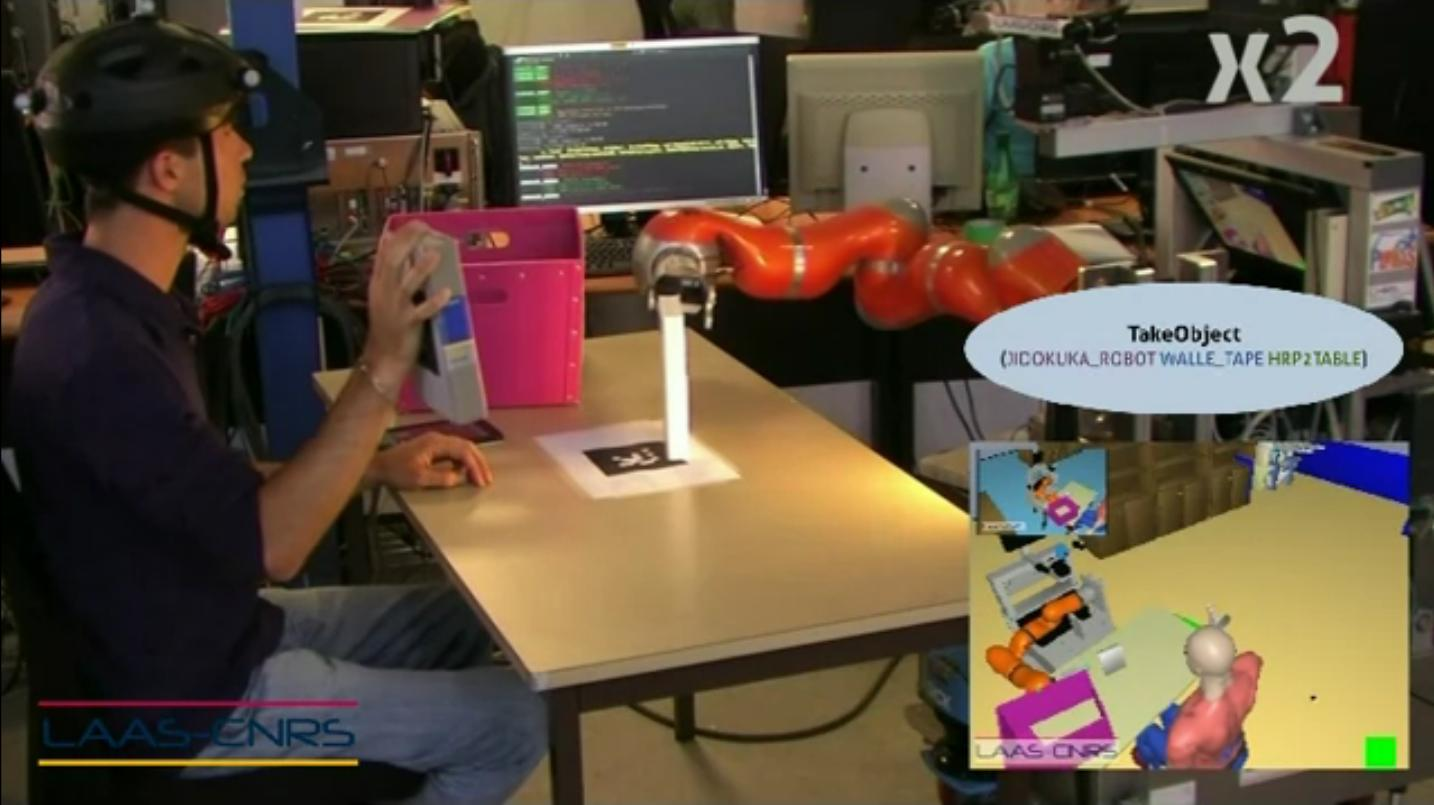
\includegraphics[width=0.6\textwidth]{cleantable.jpg}\\

        \vspace*{1em}

        \resizebox{0.7\paperwidth}{!}{%
            \begin{tikzpicture}[
                    >=latex,
                    robot/.style={fill=hriSec1CompDark!50},
                    every edge/.style={<-, draw, ultra thick},
                    every node/.style={ draw, 
                        thick,  
                        circle, 
                        font=\sf,
                        align=center,
                        node distance=2cm,
                        fill=hriSec3CompDark!50, 
                        minimum size=2cm, 
                inner sep=0.1cm}]

                \node[font=\large, draw=none, fill=none, rotate=90] at (-2, 0) {Human\\actions};
                \node[font=\large, draw=none, fill=none, rotate=90] at (-2, -3.5) {Robot\\actions};

                \node (h1) {\hatpaction{TAKE}{GREY\_TAPE}{TABLE}};
                \node[right=of h1] (h2) {\hatpaction{PUT}{GREY\_TAPE}{BIN1 }} edge (h1);

                \node[robot, below=1.5 of h1] (r1) {\hatpaction{TAKE}{BLACK\_TAPE}{TABLE }};
                \node[robot, right=of r1] (r2) {\hatpaction{PUT}{BLACK\_TAPE}{BIN2 }} edge (r1);
                \node[robot, right=of r2] (r3) {\hatpaction{TAKE}{BOTTLE}{TABLE }} edge (r2);
                \node[robot, right=of r3] (r4) {\hatpaction{PUTRV}{BOTTLE}{TABLE}} edge (r3);
                \node[robot, right=of r4] (r5) {\hatpaction{TAKE}{BOOK}{TABLE }} edge (r4);
                \node[robot, right=of r5] (r6) {\hatpaction{PUT}{BOOK}{BIN2 }} edge (r5);

                \node at (r5 |- h1) (h3) {\hatpaction{TAKE}{BOTTLE}{TABLE}} edge (h2) edge (r4);
                \node[right=of h3] (h4) {\hatpaction{PUT}{BOTTLE}{BIN1}} edge (h3);

            \end{tikzpicture}
        }

    \end{figure}

\end{frame}


\videoframe{videos/clean-table.webm?autostart}


%\subsection{The Challenge of the Real-World\texttrademark}
%\begin{frame}{Cope with the real-world}
%    \begin{enumerate}
%        \item long interaction...
%        \item ...in a human-world...
%        \item ...with humans...
%   \end{enumerate}
%\end{frame}

\videoframe[0.56]{videos/variations-splitscreen.mpg}

\videoframe{videos/roboscopie.webm?start=93}

{
\paper{Lemaignan, Gharbi, Mainprice, Herrb, Alami {\Medium Roboscopie: A Theatre Performance for a Human and a Robot} -- HRI 2012}
\begin{frame}{}
    \begin{multicols}{4}
\scriptsize

{\tt amit\_give} \\
{\tt arms\_against\_torso} \\
{\tt attachobject} \\
{\tt basicgive} \\
{\tt basicgrab} \\
{\tt basictake} \\
{\tt basket} \\
{\tt cancel\_follow} \\
{\tt cancel\_track} \\
{\tt cancel} \\
{\tt carry} \\
{\tt close\_gripper} \\
{\tt configure\_grippers} \\
{\tt detect\_and\_grab} \\
{\tt detect} \\
{\tt disabledevileye} \\
{\tt display} \\
{\tt dock} \\
{\tt enabledevileye} \\
{\tt extractpose} \\
{\tt follow} \\
{\tt glance\_to} \\
{\tt goto} \\
{\tt grab\_gripper} \\
{\tt grab} \\
{\tt gym} \\
{\tt handover} \\
{\tt handsup\_folded} \\
{\tt handsup\_folded2} \\
{\tt handsup\_folded3} \\
{\tt handsup} \\
{\tt hide} \\
{\tt idle} \\
{\tt init} \\
{\tt larm\_swinging} \\
{\tt lock\_object} \\
{\tt look\_at\_ros} \\
{\tt look\_at\_xyz} \\
{\tt look\_at} \\
{\tt looksat} \\
{\tt manipose} \\
{\tt move\_head} \\
{\tt movearm} \\
{\tt moveclose} \\
{\tt open\_gripper} \\
{\tt pick} \\
{\tt place\_agent} \\
{\tt place\_object} \\
{\tt pointsat} \\
{\tt put\_accessible} \\
{\tt put} \\
{\tt rarm\_swinging} \\
{\tt release\_gripper} \\
{\tt release} \\
{\tt restpose} \\
{\tt rotate} \\
{\tt satisfied} \\
{\tt say} \\
{\tt setpose} \\
{\tt settorso} \\
{\tt setup\_scenario} \\
{\tt show} \\
{\tt slow\_arms\_swinging} \\
{\tt sorry} \\
{\tt speed\_arms\_swinging} \\
{\tt sweep\_look} \\
{\tt sweep} \\
{\tt switch\_cameras} \\
{\tt take} \\
{\tt track\_human} \\
{\tt track} \\
{\tt translate} \\
{\tt tuckedpose} \\
{\tt unlock\_object} \\
{\tt wait} \\
{\tt waypoints} \\
    \end{multicols}
\end{frame}
}

\imageframe{croquignole.jpg}

{
\paper{Lemaignan, Hosseini, Dillenbourg {\Medium pyRobots: a Toolset for Robot Executive Control} -- IROS 2015}
\begin{frame}{}
    \centering
    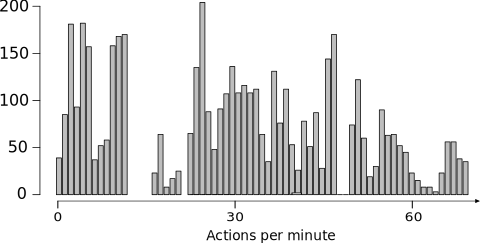
\includegraphics[width=0.8\textwidth]{actions-croquignole.pdf}

    \begin{multicols}{3}
\scriptsize
{\tt lightbar} \\
{\tt on\_toy\_added} \\
{\tt move} \\
{\tt background\_blink} \\
{\tt undock} \\
{\tt pulse\_row} \\
{\tt blink} \\
{\tt on\_lolette} \\
{\tt placeeyes} \\
{\tt on\_bumped} \\
{\tt up\_down\_row} \\
{\tt wakeup} \\
{\tt look\_at\_caresses} \\
{\tt on\_toy\_removed} \\
{\tt sneak\_in} \\
{\tt on\_lolette\_removed} \\
{\tt fall\_asleep} \\
{\tt look\_at\_lolette} \\
{\tt active\_wait} \\
{\tt closeeyes} \\
{\tt lightpattern} \\
{\tt turn} \\
{\tt idle} \\
{\tt playsound} \\
{\tt blush}

    \end{multicols}
\end{frame}
}


%%%%%%%%%%%%%%%%%%%%%%%%%%%%%%%%%%%%%%%%%%%%%%%%%%%%%%%%%%%%%%%%%%%%%%%%%%%%%%%
%\subsection{Mutual Modelling}


{
\paper{Dillenbourg, Lemaignan et al., {\Medium The Symmetry of Partner Modelling}, Intl. J. of Computer Supported Collaboratibe Learning 2016}
\begin{frame}{The False-Belief Experiment, reloaded}
    \centering
    \only<1>{
        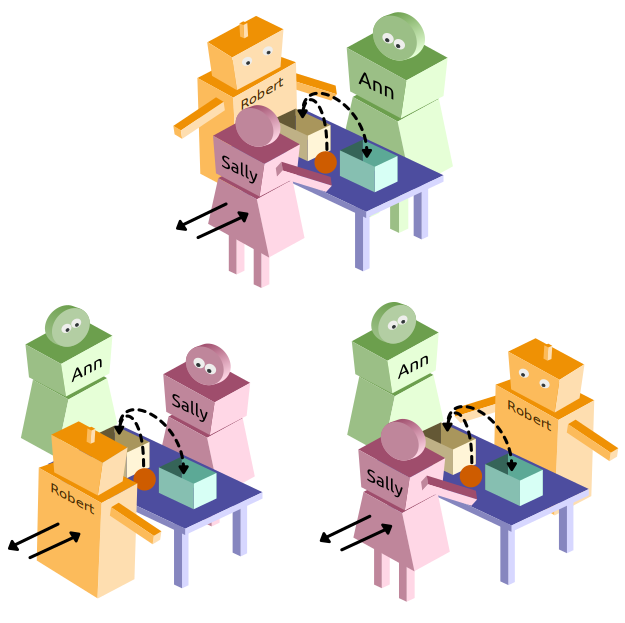
\includegraphics[width=0.7\textwidth]{triadic_false_beliefs.pdf}

    }

    \only<2>{
        \begin{multicols}{2}

            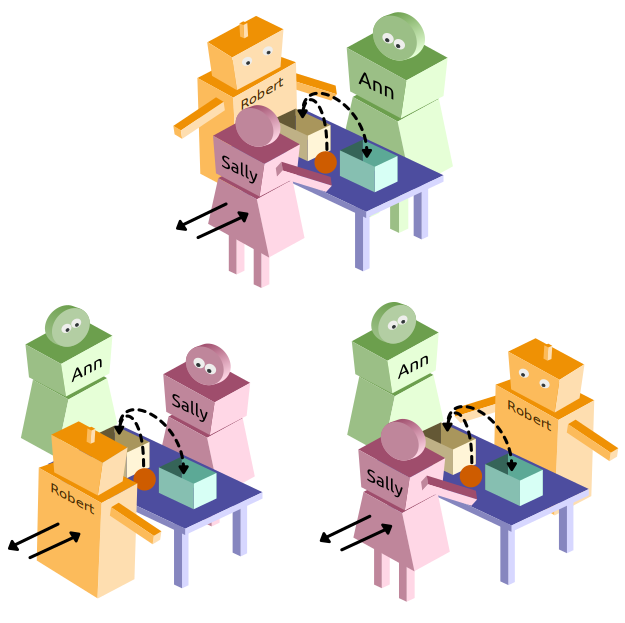
\includegraphics[width=0.9\columnwidth]{triadic_false_beliefs.pdf}

            \columnbreak

            \mbox{}\vfill

            \begin{itemize}
                \item \model{A}{B}{X}
                \item \Model{A}{B}{X}
            \end{itemize}

            \scriptsize
            e.g. {\color{hriSec1} \model{\text{robot}}{\text{Sally}}{plans}}

            \vfill\mbox{}

        \end{multicols}
    }

    \only<3>{
        \begin{itemize}
            \item {\Medium Robot is the observer}\\
                \Model{R}{\text{Sally}|\text{Ann}}{plans}? can the human
                verbalise it? i.e. \model{H}{R}{\Mmodel{R}{H}{plans}}?

            \item {\Medium Robot is an active participant}\\
                \model{H}{R}{knowledge|plans|goals}? i.e. How Ann interprets the
                behaviour of a robot who moves the ball from the beige box to
                the blue box while Sally is away?

        \end{itemize}
    }
    \only<4>{
        \begin{multicols}{2}
            \vspace*{0.4cm}
            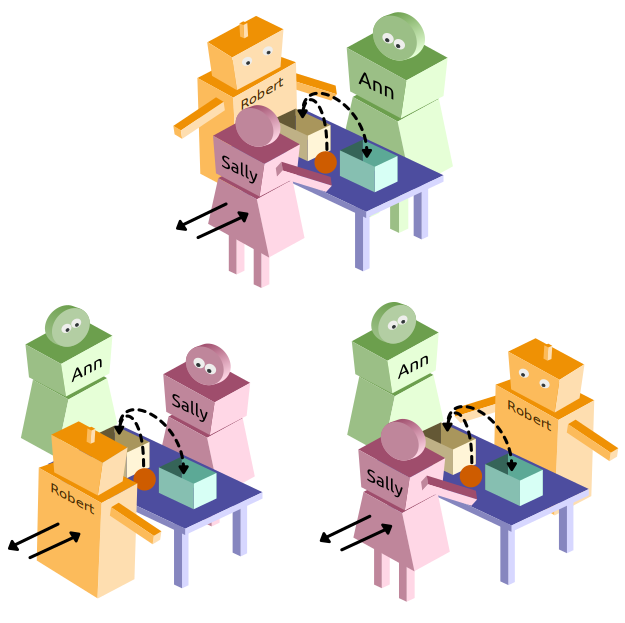
\includegraphics[width=0.9\columnwidth]{triadic_false_beliefs.pdf}



            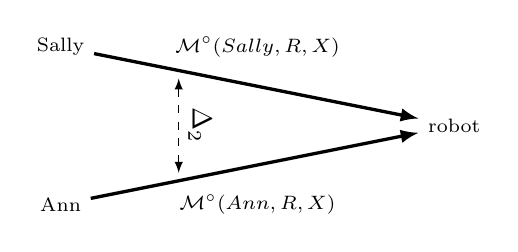
\begin{tikzpicture}[
                    >=latex,
                scale=0.5]

                \draw(0,2) node (A) {\scriptsize Sally};
                \draw(0,-2) node (B) {\scriptsize Ann};
                \draw(10,0) node (C) {\scriptsize robot};

                \draw(5,2) node {\scriptsize \Model{Sally}{ R}{ X}};
                \draw(5,-2) node {\scriptsize \Model{Ann}{ R}{ X}};
                \draw[dashed, <->] (3,1.2) -- (3,-1.2) node[midway, sloped, above] {$\Delta_2$};
                \draw[->,very thick] (A) to (C);
                \draw[->,very thick] (B) to (C);

            \end{tikzpicture}

            \vspace*{1cm}

            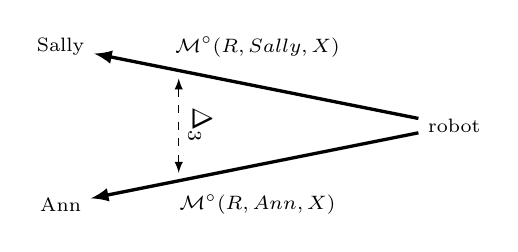
\begin{tikzpicture}[
                    >=latex,
                scale=0.5]

                \draw(0,2) node (A) {\scriptsize Sally};
                \draw(0,-2) node (B) {\scriptsize Ann};
                \draw(10,0) node (C) {\scriptsize robot};

                \draw(5,2) node {\scriptsize \Model{R}{ Sally}{ X}};
                \draw(5,-2) node {\scriptsize \Model{R}{ Ann}{ X}};
                \draw[dashed, <->] (3,1.2) -- (3,-1.2) node[midway, sloped, above]
                {$\Delta_3$};
                \draw[<-,very thick] (A) to (C);
                \draw[<-,very thick] (B) to (C);

            \end{tikzpicture}
        \end{multicols}
    }
    \only<5>{
        Do Sally and Ann have the same accuracy when modelling the robot?

        {\centering
            \(\Delta_2 = \Delta(\Mmodel{\text{Sally}}{R}{X}, \Mmodel{\text{Ann}}{R}{X})\)

        }

        \vspace*{1em}
        Conversely, what may lead the robot to model more accurately
        Sally or Ann?

        {\centering
            \(\Delta_3= \Delta(\Mmodel{R}{\text{Sally}}{X}, \Mmodel{R}{\text{Ann}}{X})\)

        }

    }
\end{frame}

\end{document}
